%%%%%%%%%%%%%%%%%%%%%%%%%%%%%%%%%%%%%%%%%%%%%%%
% LATEX UT THESIS TEMPLATE 							      	   	 %
% By Elahe Rannai									        	 %
% No rights reserved. The author appreciates any distribution and/or completion of this material.  	 %
%%%%%%%%%%%%%%%%%%%%%%%%%%%%%%%%%%%%%%%%%%%%%%%
\documentclass[twoside, a4paper,11pt]{book}
\usepackage[margin=10mm,font={footnotesize},labelfont={footnotesize}]{caption}

\usepackage{amsmath}
\usepackage{graphicx}
\usepackage[multidot]{grffile}
\usepackage{wrapfig}
\usepackage{verbatim}
\usepackage{fancyhdr}
\usepackage{url}
\usepackage{hyperref}
\usepackage{supertabular}
\usepackage{multicol}
\usepackage{setspace}
\usepackage{changepage}
\usepackage{color}
\usepackage{array}
\usepackage{colortbl}

\usepackage{amsmath}
\usepackage{amsthm}
\usepackage{amssymb}
\usepackage{cancel}
\usepackage{mathtools}
\usepackage{extpfeil}

\usepackage{subfigure}
\usepackage{tabularx}
\usepackage{multirow}
\usepackage{afterpage}
\usepackage{pdfpages}

\usepackage{cite}
%\usepackage{cleveref}
\usepackage[rgb,x11names]{xcolor}% Optimize for screen reading.


\usepackage{algorithm}
\usepackage{algorithmic}
\usepackage[xindy]{glossaries}

\usepackage{zref-abspage}
\usepackage{perpage}
\MakePerPage{footnote}

\usepackage{hhline}
\usepackage[T1]{fontenc}
\usepackage{xcolor}    % loads also »colortbl«
\usepackage[export]{adjustbox}

\usepackage[extrafootnotefeatures]{xepersian}
\LTRcolumnfootnotes


\numberwithin{equation}{chapter}
\numberwithin{table}{chapter}
\numberwithin{figure}{chapter}
\numberwithin{equation}{chapter}


\settextfont[Scale=1.12]{XB Niloofar}
\setlatintextfont[Scale=1.05]{Times New Roman}

\DefaultMathsDigits
\DeclareMathSizes{10}{12}{8}{6}   % For size 10 text


\defpersianfont\nastaliq[Scale=1]{IranNastaliq}
\defpersianfont\nastaliqbig[Scale=1.3]{IranNastaliq}


\linespread{2.04}
\setlength\parskip{0.25cm}
\setlength\topmargin{-0.5in}
\setlength\headheight{2cm}
\setlength\headsep{0.7cm}
\setlength\textheight{8.997in}
\setlength\textwidth{5.9078in}
\setlength\oddsidemargin{-0.0158in}
\setlength\evensidemargin{0.38in}

\setlength{\parindent}{1cm}

\newenvironment{strict_enumerate}
{\begin{enumerate}
  \setlength{\itemsep}{0.1pt}
  \setlength{\parskip}{0pt}
  \setlength{\parsep}{0pt}}
{\end{enumerate}}

\newenvironment{strict_itemize}
{\begin{itemize}
  \setlength{\itemsep}{1pt}
  \setlength{\parskip}{0pt}
  \setlength{\parsep}{0pt}}
{\end{itemize}}


\newenvironment{strict_description}
{\begin{description}
  \setlength{\itemsep}{1pt}
  \setlength{\parskip}{0pt}
  \setlength{\parsep}{0pt}}
{\end{description}}


\newglossarystyle{mylistFa}{
\glossarystyle{list}
\renewenvironment{theglossary}{}{}
\renewcommand*{\glossaryheader}{}
\renewcommand*{\glsgroupheading}[1]{}
\renewcommand*{\glsgroupskip}{}
\renewcommand*{\glossaryentryfield}[5]     {\noindent\glstarget{##1}{##2}\dotfill \space \lr{##3} \\}
\renewcommand*{\glossarysubentryfield}[6]{\glossaryentryfield{##2}{##3}{##4}{##5}{##6}}
}

\newglossarystyle{mylistLa}{
\glossarystyle{list}
\renewenvironment{theglossary}{}{}
\renewcommand*{\glossaryheader}{}
\renewcommand*{\glsgroupheading}[1]{}
\renewcommand*{\glsgroupskip}{}
\renewcommand*{\glossaryentryfield}[5]     {\noindent\glstarget{##1}{##3}\dotfill \space ##2 \\}
\renewcommand*{\glossarysubentryfield}[6]{\glossaryentryfield{##2}{##3}{##4}{##5}{##6}}
}

\newglossary[glg]{latin}{gls}{glo}{واژه‌نامه‌ انگلیسی به فارسی}
\newglossary[blg]{persian}{bls}{blo}{واژه‌نامه‌ فارسی به انگلیسی}

\newcommand{\mls}[1]{\gls{fa-#1}\glsuseri{la-#1}}

\newcommand{\inpdic}[2]{
	\newglossaryentry{fa-#1}{type=persian,name={#1}, sort={#1},description={#2}}
	\newglossaryentry{la-#1}{type=latin,name=\lr{#2}, sort={#2},description={#1}}
}


\makeatletter
\renewcommand*{\cleardoublepage}{\clearpage\if@twoside \ifodd\c@page\else
\hbox{}%
\thispagestyle{empty}%
\newpage%
\if@twocolumn\hbox{}\newpage\fi\fi\fi}

%meee error ! LaTeX Error: \gls@persian@displayfirst undefined.
%\renewcommand{\gls@persian@displayfirst}[4]{
	%#1#4\protect\LTRfootnote{#2}
%}
\defglsdisplayfirst[persian]{#1#4\protect\LTRfootnote{#2}}

%\makeatother
\makeglossaries
\glsdisablehyper
\inpdic{بازی‌های شناختی}{Cognitive Games}
\inpdic{توانایی‌های شناختی}{Cognitive Abilities}
\inpdic{تمرین‌های شناختی}{Cognitive training}
\inpdic{توجه و تمرکز}{Attention}
\inpdic{توجه}{Attention}
\inpdic{حافظه}{Memory}
\inpdic{حل مساله}{Problem Solving}
\inpdic{استراتژی}{Strategy}
\inpdic{استراتژی یادگیری}{Learning Strategy}
\inpdic{راهبرد}{Strategy}
\inpdic{راهبرد یادگیری}{Learning Strategy}
\inpdic{تکرار کردن}{Rehearsal}
\inpdic{برقرار کردن ارتباط معنایی}{Semantic}
\inpdic{گروه کردن}{Grouping}
\inpdic{تماس چشمی}{Eye contact}
\inpdic{توضیح دادن}{Paraphrasing}
\inpdic{گفتگو با خود}{self-talk}
\inpdic{توجه تقسیم شده}{Divided Attention}
\inpdic{ردیابی همزمان چندین شیء}{Multiple Object Tracking}
\inpdic{ادراک}{Perception}
\inpdic{مهارت‌های حرکتی}{Motor Skills}
\inpdic{کارکردهای اجرایی}{Executive Functions}
\inpdic{بیش‌فعالی}{ADHD}
\inpdic{اختلال کمبود توجه}{ADD}
\inpdic{فعالیت‌ها}{task}
\inpdic{شرکت‌کننده}{subject}
\inpdic{حافظه‌ی کاری}{Working Memory}
\inpdic{هوش سیال}{Fluid Intelligence}
\inpdic{انجام چند کار همزمان}{Multitasking}
\inpdic{ظرفیت حافظه‌ی کاری}{Working Memory Capacity}
\inpdic{هوش متبلور}{Crystallized Intelligence}
\inpdic{انگیزه}{Motivation}
\inpdic{انتقال}{transfer}
\inpdic{مقاومت در برابر چالش}{Persistence}
\inpdic{تجسم فضایی}{Spatial Skills}
\inpdic{آموزش استراتژی}{Strategy training}
\inpdic{آموزش راهبرد}{Strategy training}
\inpdic{حافظه‌ی کاری کلامی}{Verbal working memory}
\inpdic{درک مطلب شنیداری}{Passage listening comprehension}
\inpdic{منحرف کننده}{distractor}
\inpdic{حرکات چشم}{saccade}
\inpdic{مبتنی بر مدل}{model-based}
\inpdic{غیر مبتنی بر مدل}{model-free}
\inpdic{آزمون دو مرحله‌ای دا}{daw two step task}
\inpdic{قدم زدن تصادفی}{random walk}
\inpdic{بدنه‌ی محدب}{convex hull}
\inpdic{دمای معکوس}{inverse temperature}
\inpdic{نمودار احتمال نرمال بودن}{normal probability plot}
\inpdic{داده‌های پرت}{outliers}
\inpdic{یادگیری ماشین}{machine learning}
\inpdic{یادگیری تقویتی}{reinforcement learning}
\inpdic{میانه انحراف مطلق}{median absolute deviation}
\inpdic{پیرسون}{Pearson}
\inpdic{نمودار نقطه‌ای}{scatter plot}
\inpdic{ویلکاکسون}{Wilcoxon}
\inpdic{کروسکال-والیس}{Kruskal-Wallis}
\inpdic{هیستوگرام}{Histogram}
\inpdic{تیم مغزینه}{maghzineh.com}
\inpdic{توجه پایدار}{Sustained Attention}
\inpdic{توجه انتخابی}{Selective Attention}
\inpdic{توجه متناوب}{Alternating Attention}
\inpdic{توجه تقسیم‌شده}{Divided Attention}
\inpdic{برخط}{online}
\inpdic{منحرف‌کننده}{distractor}
\inpdic{آنالیز واریانس}{ANOVA}
\inpdic{کولموگروف-اسمیرنف}{Kolmogorov–Smirnov}
\inpdic{پیشین}{pre-test}
\inpdic{پسین}{post-test}



\begin{document}
% Besmellah Page
\newpage
\thispagestyle{empty}
\begin{center}
\begin{tabular}{c}
\\ \\ \\ \\ \\

\includegraphics[scale=0.7, origin=c]{Figures/besm1.jpg}\\
\end{tabular}
\end{center}
%


\newpage
\thispagestyle{empty}
\mbox{}

%%%%%%%%%%%%%%%%%
%TITLE PAGE
%%%%%%%%%%%%%%%%%
\newpage
\thispagestyle{empty}
\begin{center}
\begin{tabular}{lp{7cm}r}

\includegraphics[width=2.8cm]{Figures/ut.png} & & 
\includegraphics[width=3.8cm]{Figures/eng.png} \\
\end{tabular}

{\LARGE\bfseries دانشگاه \space تهران}
\\*
{\Large\bfseries پردیس دانشکده‌های فنی}
\\*
{\Large\bfseries دانشکده‌ مهندسی برق و کامپیوتر}
\par
\vskip 1.4cm
{\Huge\bfseries ارزیابی تجربه‌ی کاربران در بازی شناختی توجه و استفاده از آنها برای بهبود عملکرد افراد مبتدی}\par
\vskip .9cm
{\large%
  نگارش }\par
{\Large\bfseries الهه ابوالحسنی شهرضا}\par
\par
{\large
  اساتید راهنما\par
\Large\bfseries دکتر مجید نیلی  \\
\Large\bfseries دکتر هادی مرادی  \\

}
\par
\vskip 1.4cm
{\large\bfseries پایان‌نامه برای دریافت درجه کارشناسی‌ارشد در رشته \\* مهندسی کامپیوتر - گرایش هوش مصنوعی}
\par
\vskip .5cm
{\large شهریور ۱۳۹۶}
\par
\vfill
\end{center}

%%%%%%%%%%%%%%%%%%%%
%\newpage
%\thispagestyle{empty}
%\mbox{}

%\newpage
%\thispagestyle{plain}
%\begin{center}
%\begin{tabular}{lp{7cm}r}
%\includegraphics[width=15cm]{Figures/Table.png} 
%\end{tabular}
%\end{center}
%%%%%%%%%%%%%%%%%%%%%%
\newpage
\thispagestyle{empty}
\mbox{}

\newpage
\thispagestyle{plain}
\begin{center}
\begin{tabular}{lp{7cm}r}

\includegraphics[width=2.8cm]{Figures/ut.png} & & 
\includegraphics[width=3.8cm]{Figures/eng.png} \\
\end{tabular}

{\LARGE\bfseries دانشگاه \space تهران}
\\*
{\Large\bfseries پردیس دانشکده‌های فنی}
\\*
{\Large\bfseries دانشکده مهندسی برق و کامپیوتر}
\par
پایان نامه برای دریافت درجه کارشناسی ارشد در رشته مهندسی کامپیوتر

\vskip 1cm
\par
عنوان:

{\Large\bfseries ارزیابی تجربه‌ی کاربران در بازی شناختی توجه و استفاده از آنها برای بهبود عملکرد افراد مبتدی}

\vskip .2cm
{\Large نگارش: الهه ابوالحسنی شهرضا}
\end{center}
\vskip .3cm

\noindent
این پایان‌نامه در تاریخ ۱۳۹۶/۰۶/۱۲ در مقابل هیأت داوران دفاع گردید و مورد تصویب قرار گرفت.
\vskip .5cm
\begin{tabular}{r r}
معاون آموزشی و تحصیلات تکمیلی پردیس دانشکده‌های فنی: دکتر جلیل آقا راشد محصل \\
رئیس دانشکده مهندسی برق و کامپیوتر: دکتر مجید نیلی\\
معاون پژوهشی و تحصیلات تکمیلی: دکتر بابک نجار اعرابی \\
استاد راهنما: آقای دکتر مجید نیلی \\
استاد راهنمای دوم: آقای دکتر هادی مرادی\\
عضو هیأت داوران:  \\
عضو هیأت داوران:  \\

\end{tabular}



\newpage
\thispagestyle{empty}
\mbox{}

\newpage
\thispagestyle{empty}
{ \LARGE 
\begin{center}
تعهدنامه اصالت اثر
\end{center}}
اینجانب الهه ابوالحسنی شهرضا تایید می‌کنم که مطالب مندرج در این پایان نامه حاصل کار و پژوهش اینجانب بوده و به دستارود‌های پژوهشی دیگران که در این نوشته از آنها استفاده شده است مطابق مقررات ارجاع گردیده است. به‌علاوه این پایان نامه قبلا برای احراز هیچ مدرک هم سطح یا بالاتر ارائه نشده است.
\par
کلیه حقوق مادی و معنوی این اثر متعلق به دانشکده فنی دانشگاه تهران است.
\par 
\vskip 2cm


\begin{flushleft}
نام و نام خانوادگی دانشجو: الهه ابوالحسنی شهرضا \hspace{1.75cm}~~~~~~~ \\
امضای دانشجو: ~~~~~~~~~~~~~~~~~~~~~~~~~~~~~~~~~~~~~~~~~~~~~~~~~~~~~
\end{flushleft}

\newpage
\thispagestyle{empty}
\mbox{}


%\newpage
%\thispagestyle{empty}
%\mbox{}
%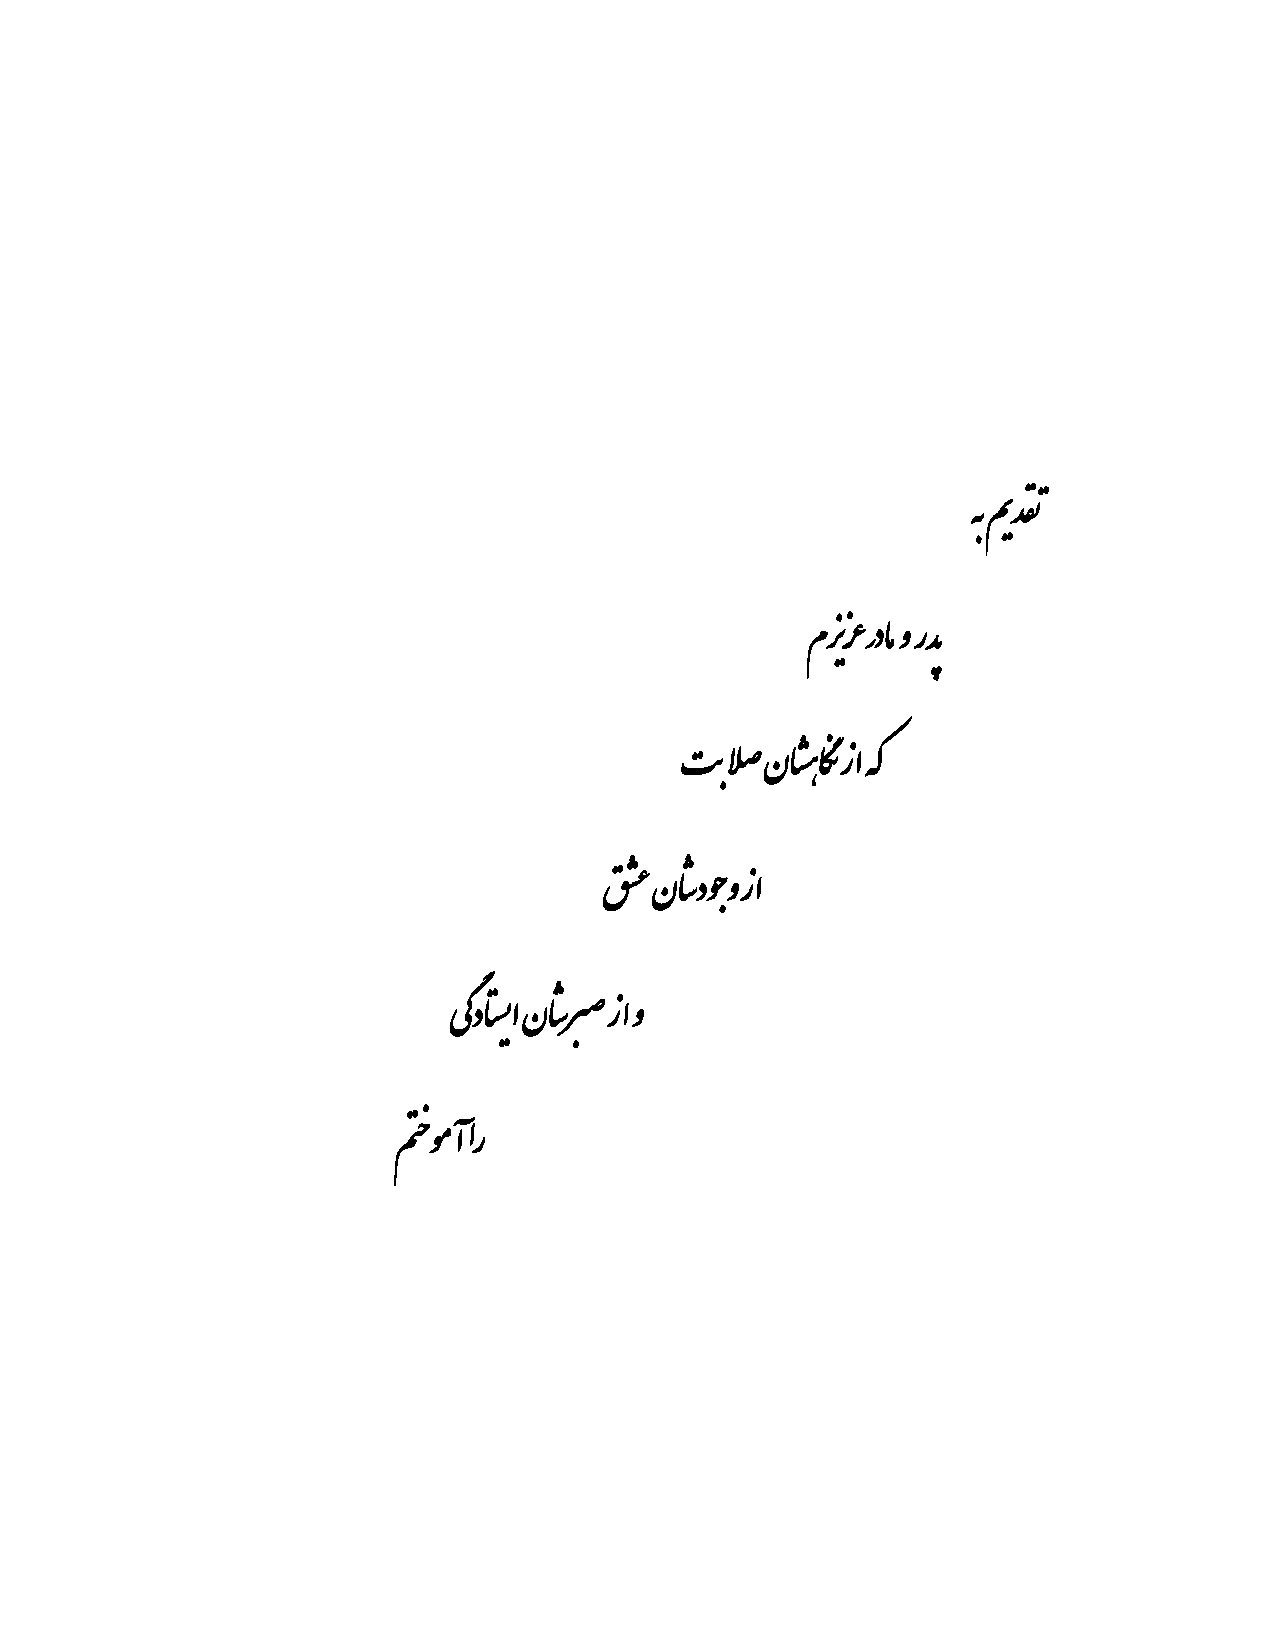
\includegraphics[scale=0.9]{Figures/taghdir.pdf} 


\newpage
\thispagestyle{empty}
\mbox{}


\newpage
\thispagestyle{empty}
{\nastaliqbig \Huge 
تقدیر و تشکر\nastaliq

{\par\vspace{1cm}}
\LARGE
\begin{adjustwidth}{1cm}{}
مراتب تشکر و قدردانی خود را نسبت به تمام کسانی که مرا در انجام این پایان‌نامه یاری کرده‌اند، خصوصاً اساتید گرامی و ارجمندم، جناب آقای دکتر نیلی و جناب آقای دکتر مرادی که رهنمودهای ایشان همواره راهگشای پیچیدگی‌های این پژوهش بوده است، ابراز می‌دارم. 

همچنین، از تمامی دوستانم در آزمایشگاه رباتیک شناختی که با حضور و محبتشان مرا یاری نمودند تشکر و قدردانی می‌نمایم. 

\end{adjustwidth}
}


\newpage
\thispagestyle{empty}
\mbox{}


\pagestyle{plain}

\newpage


\vspace*{-2.6cm}
\subsection*{چکیده}

\vspace*{-.4cm}

\begin{spacing}{1.5}

در سال‌های اخیر گروه‌های زیادی اقدام به طراحی و توسعه‌ی بازی‌های شناختی کامپیوتری کرده‌اند که هدف آن کمک به ارتقاء توانمندی‌های شناختی مانند توجه و تمرکز، حافظه و حل مساله است. لیکن نتیجه‌ی مطالعات بر روی اثربخشی این بازی‌ها در ارتقاء قابلیت‌های شناختی متناقض است. این تناقض در پاسخ به این سوال است که آیا راهبردهای خودیافته که افراد جهت بهبود عملکردهای شناختی خود در محیط بازی از آن استفاده می‌کنند، قابل تعمیم به دنیای واقعی نیز است یا به محیط بازی منحصر می‌شود. 

با در نظر گرفتن این موضوع که استفاده‌ی آگاهانه از یک راهبرد، احتمال استفاده از آن را در دنیای واقعی بیشتر می‌کند در این پژوهش بر آنیم که به دو سوال اساسی پاسخ دهیم. نخست آن که  آیا تفاوت بین عملکرد افراد، در اثر استفاده‌ی آنها از راهبردهای متفاوت ایجاد می‌شود یا ناشی از تفاوت در ویژگی‌های فردی آنهاست. دیگر آن که در صورت یافتن یک یا چند راهبرد موثر، آیا این راهبرد قابلیت آموزش دارد و منجر به اثربخشی بیشتر در بازی می‌شود یا خیر. در ذیل سوال نخست به دو موضوع پرداخته می‌شود. موضوع اول جمع‌آوری راهبردهای مورد استفاده افراد و موضوع دوم استخراج راهبردهای موثر است. برای این کار از یک بازی شناختی توسعه داده شده توسط مجموعه‌ی مغزینه در حوزه‌ی «توجه تقسیم شده» استفاده شد که ویژگی‌ها و مراحل آن متناسب با نیازهای پژوهش بازطراحی شدند. از افراد خواسته شد در مدت زمان محدود بازی نموده و راهبردهای مورد استفاده‌ی خود را با استفاده از پرسشنامه گزارش کنند. آزمون تا جایی ادامه پیدا می‌کند که راهبرد جدیدی گزارش نشود. برای استخراج راهبردها از پرسشنامه‌ها، از روش تحلیل محتوا و کدگذاری پاسخ‌ها استفاده شد. سپس با استفاده از روش‌های آماری نمره‌ی هر کدام از راهبردها محاسبه شد. در نهایت راهبردهای به دست آمده به سه گروه اصلی تقسیم‌بندی شدند و مشخص شد یکی از این سه گروه نسبت به دو گروه دیگر اثربخشی بیشتری دارد. در ادامه برای پاسخ به سوال اصلی دوم، دو موضوع بررسی شدند. اول اینکه ارتباط میان میزان یادگیری راهبرد و بهبود عملکرد افراد به چه صورت است و دوم اینکه این میزان چه ارتباطی با مدل محور یا مدل آزاد بودن روش یادگیری فرد دارد. برای پاسخ دادن به این سوالات یک آزمون سه مرحله‌ای طراحی شد که در  مرحله اول میزان مدل محور بودن یادگیری فرد معلوم می‌شود. در دو مرحله‌ی بعدی از بازی بخش اول استفاده می‌شود. در  مرحله دوم، بازی انجام شده و راهبردها توسط افراد گزارش می‌شوند. سپس راهبردهای موثرتر به دو صورت کلامی و با استفاده از راهنمای داخل بازی آموزش داده می‌شود. در نهایت در مرحله سوم بازی مجدداً تکرار شده و از فرد خواسته می‌شود میزان استفاده از راهبرد آموزش داده شده را گزارش کند. در کنار این آزمون یک آزمون دو مرحله‌ای از گروه کنترل گرفته می‌شود که فاقد مرحله‌ی اول و آموزش راهبرد است. این مراحل بدون وقفه و پشت سر هم انجام می‌شوند. 

در نتایج به دست آمده مشاهده می‌کنیم ارتباط معناداری بین مدل محور بودن فرد و میزان یادگیری راهبرد وجود ندارد. همچنین بهبود عملکرد افرادی که راهبرد به آنها آموزش داده نشده به طرز معناداری بیشتر از افرادی است که راهبرد به آنها آموزش داده شده است.

\textbf{واژه‌های کلیدی: }\textit{راهبرد، بازی شناختی، توجه و تمرکز، توجه تقسیم‌شده، مدل محور}
\end{spacing}

\pagenumbering{harfi}


\newpage
\thispagestyle{empty}
\mbox{}

\renewcommand\listfigurename{فهرست شکل‌ها}
\renewcommand\listtablename{فهرست جدول‌ها}
%\renewcommand{\refname}{مراجع}

\begin{doublespace}\small{
\tableofcontents
\listoftables
\listoffigures
}\end{doublespace}





\pagestyle{fancy}	
\fancyhead{} 
\fancyhead[RO]{\leftmark}
\fancyhead[LO]{\thepage}
\fancyhead[LE]{\rightmark}
\fancyhead[RE]{\thepage}
\fancyfoot{} 
\renewcommand{\headrulewidth}{0.6pt} 
\renewcommand{\footrulewidth}{0pt}

\chapter{مقدمه}
\label{chapter:introduction}
\pagenumbering{arabic}\setcounter{page}{1}
\thispagestyle{plain}

بسیاری از ما در زندگی روزمره با موقعیت‌هایی روبرو می‌شویم که مطلبی را که باید به خاطر بیاوریم فراموش می‌کنیم، هنگام رانندگی حواسمان پرت می‌شود و باعث بروز حادثه می‌شویم یا نمی‌توانیم راجع به انتخاب مسیر تصمیم بگیریم. همه‌ی ما با چنین موقعیت‌ها و موقعیت‌های مشابه دیگر برخورد کرده‌ایم. برای غلبه کردن بر چنین موقعیت‌هایی نیاز داریم برخی از توانایی‌های بنیادین خود را تقویت کنیم. این توانایی‌ها پایه و اساس بسیاری از کارهایی هستند که به صورت روزمره انجام می‌دهیم. به این توانایی‌ها \mls{توانایی‌های شناختی} گفته می‌شود. در مثال‌های بالا برای به خاطر سپردن موضوعات مختلف باید حافظه‌ی خود را تقویت کنیم. برای رانندگی بهتر باید توانایی توجه خود را بهبود بخشیم و برای انتخاب مسیر باید بتوانیم تصمیم‌گیری موثر داشته باشیم. 

توانایی‌های شناختی، مانند سایر ویژگی‌های انسان، همزمان با رشد او ظهور و بروز پیدا می‌کنند و سپس با کهولت سن کم کم دچار نقصان می‌شوند. همانطور که از جسم خود مراقبت می‌کنیم و با ورزش کردن و تغذیه‌ی سالم تلاش می‌کنیم فرآیند پیر شدن را به تعویق بیاندازیم باید هوشیار سلامت مغز خود نیز باشیم. مغز ما نیز مانند جسم‌مان به مرور زمان قابلیت‌های خود را از دست می‌دهد. همچنین ممکن است با بروز یک حادثه برخی از فعالیت‌های مغزی‌مان دچار مشکل شود. توانایی‌های شناختی نیز بخشی از قابلیت‌های مغز ما هستند که ممکن است تحت تاثیر این موضوعات قرار بگیرند.

یکی از روش‌های بهبود قابلیت‌های مغزی و توانایی‌های شناختی تمرین دادن آنهاست. از مدت‌ها قبل، از تمرین‌های فیزیکی یا قلم و کاغذی برای بهبود مشکلات ذهنی برخی از افراد استفاده می‌شده است. به عنوان مثال می‌توان به افرادی اشاره کرد که در اثر حادثه دچار آسیب شده‌اند \cite{carney1999TBI}، افراد مسنی که توانایی‌های شناختی‌شان تحلیل رفته است \cite{rapp2002olderAdults}، کودکانی که دچار آسیب‌هایی مانند نقص توجه یا بیش فعالی بوده‌اند یا مشکلاتی مانند اختلال یادگیری داشته‌اند \cite{kimberly1999ADHDKids}. متناسب با نوع آسیب، شدت آن و سن فرد تمرین‌هایی تعیین می‌شود که منجر به کاهش روند تخریب یا بهبود ناحیه‌ی آسیب دیده شود. به چنین تمرین‌هایی  \mls{تمرین‌های شناختی} گفته می‌شود. این تمرین‌ها در واقع نوعی ورزش مغزی هستند که در بسیاری از موارد، به ویژه هنگام کار با کودکان، به صورت بازی ارائه می‌شوند.

با پیشرفت تکنولوژی و گسترش آن در تمام ابعاد زندگی بشر، حوزه‌ی تمرین‌های شناختی نیز دچار تغییر و تحول شده است. سازمان‌های بسیاری (مانند \lr{lumosity.com} و \lr{fitbrains.com}) اقدام به طراحی و توسعه‌ی تمرین‌های شناختی کامپیوتری کرده‌اند و این تمرین‌ها را در قالب بازی ارائه می‌دهند. این پیشرفت باعث شده است تمرین‌ها و بازی‌های شناختی به صورت گسترده در دسترس تمامی افراد قرار بگیرند و حتی افراد عادی نیز بتوانند به راحتی از این امکانات استفاده کنند. 

اما سوالی که به وجود می‌آید این است که واقعا چقدر این تمرین‌ها باعث تقویت توانایی‌های شناختی و قابلیت‌های مغز ما می‌شوند. در مورد افرادی که دچار آسیب هستند تاثیرگذاری تمرین‌های شناختی اثبات شده است (\cite{carney1999TBI}، \cite{rapp2002olderAdults}، \cite{kimberly1999ADHDKids}). اما برای افراد عادی آیا همانطور که بسیاری از ارائه دهندگان این بازی‌ها ادعا می‌کنند، تمرین‌ها تاثیرگذار هستند و باعث بهبود توانایی‌های شناختی در زندگی واقعی می‌شوند یا صرفا با بازی کردن می‌توانیم عملکرد خود در بازی مورد نظر را بهبود بخشیم؟ این موضوع توسط پژوهشگران مختلفی بررسی شده است. (\cite{melby2013WM}، \cite{redick2013Intellig}) ولی نتایج به دست آمده توسط آنان با یکدیگر متفاوت است. برخی از این پژوهش‌ها مدعی هستند این بازی‌ها تاثیرگذاری طولانی مدت و در زندگی واقعی دارند و برخی دیگر می‌گویند تاثیراتشان تنها کوتاه مدت و در حوزه‌ی بازی است. با توجه به این تناقض یکی از مسائلی که بررسی می‌شود عوامل موثر در تاثیرگذاری بازی‌های شناختی است. این عوامل می‌توانند شامل تفاوت‌های فردی و غیرفردی شوند \cite{jaeggi2013IndiDiff}. تفاوت‌های فردی شامل ویژگی‌هایی مانند سن، ویژگی‌های شناختی و باور بازیکن راجع به موضوعات مختلف است. تفاوت‌های غیرفردی شامل موضوعاتی مانند محیط انجام بازی و ویژگی‌های بازی هستند.

یکی از ویژگی‌های فردی که افراد مختلف را متفاوت می‌کند روشی است که هنگام بازی کردن از آن استفاده می‌کنند. سوالی که ایجاد می‌شود این است که آیا افرادی که عملکرد شناختی بهتری دارند از روش‌های متفاوتی برای انجام دادن فعالیت‌های خود استفاده می‌کنند؟ یا این تفاوت، نشات گرفته از تفاوت‌های ذاتی آنها است؟ به این روش‌ها در این پژوهش \mls{راهبرد} گفته می‌شود. اگر پاسخ سوال اول مثبت باشد در ادامه این سوال را می‌پرسیم که آیا می‌توان با آموزش راهبرد افراد حرفه‌ای به افراد مبتدی باعث بهبود عملکرد آنها شد؟ از این روش در حوزه‌های مختلف، مانند آموزش زبان دوم (\cite{oxford1989LangStrategy})  یا بهبود عملکرد دانشگاهی (\cite{donker2014Academic}) استفاده می‌شود و به آن \mls{آموزش راهبرد} گفته می‌شود. در حوزه‌ی بازی‌های شناختی حافظه نیز از این روش بسیار استفاده شده است و راهبردهای شناخته‌شده‌ی  زیادی در این حوزه وجود دارد. به عنوان مثال می‌توان به  \mls{تکرار کردن} ، \mls{برقرار کردن ارتباط معنایی} یا \mls{گروه کردن} اشاره کرد \cite{morrison2016WM}. بسیاری از ما هنگام درس خواندن به صورت آگاهانه یا ناآگاهانه از برخی از این راهبردها استفاده کرده‌ایم.

با توجه به اهمیت موضوع «توجه» به عنوان یکی از توانمند‌ی‌های شناختی، در این پژوهش هدف نهایی بهبود عملکرد افراد در یک بازی شناختی «توجه» با استفاده از آموزش راهبرد است. معمولا این حوزه را به چهار زیرشاخه‌ی اصلی تقسیم‌بندی می‌کنند: \mls{توجه پایدار}، \mls{توجه انتخابی}، \mls{توجه متناوب} و \mls{توجه تقسیم‌شده}. توجه پایدار زیرشاخه‌ای از توجه است که در آن لازم است به یک موضوع به مدت طولانی توجه کنیم. توجه انتخابی وقتی مورد استفاده قرار می‌گیرد که نیاز داریم به یک فعالیت از میان فعالیت‌های مختلف توجه کنیم. توجه متناوب زمانی اهمیت پیدا می‌کند که لازم باشد توجه‌مان بین چند فعالیت به صورت متناوب عوض شود و توجه تقسیم‌شده مربوط به شرایطی است که لازم است به چند فعالیت به صورت همزمان توجه کنیم. به عنوان مثال در شرایطی که سعی می‌کنیم در حال رانندگی کردن به عابر پیاده و به ماشینی که در حال نزدیک شدن به ماست همزمان توجه کنیم در حال استفاده کردن از توانایی توجه تقسیم شده هستیم. 

راهبردهای مربوط به توجه تا به امروز کمتر بررسی شده‌اند. از راهبرد‌های شناخته شده در حوزه‌ی توجه می‌توان به \mls{تماس چشمی} ، \mls{توضیح دادن} یا \mls{گفتگو با خود} اشاره کرد \cite{twamley2008CogTrain}.\\ مهم‌ترین تمایز این پژوهش با کارهایی که تا کنون انجام شده، انتخاب حوزه‌ی «توجه» است. در این پژوهش سعی شده است مجموعه‌ای از راهبرد‌های مربوط به «\mls{توجه تقسیم شده}» معرفی شوند. به منظور دستیابی به این هدف یک بازی شناختی با نام «ابر باران‌زا» انتخاب شد که هدف اصلی آن بهبود شاخه‌ی «توجه تقسیم‌شده» است. این بازی الهام گرفته از فعالیت «ردیابی همزمان چند شیء» است. روشی که برای بهبود عملکرد افراد استفاده می‌شود آموزش راهبرد است. آگاهی نسبت به راهبرد باعث می‌شود افراد بتوانند علاوه بر بازی، در زندگی واقعی نیز از آن استفاده کنند و در نتیجه تاثیرگذاری بازی‌ها تنها منحصر به محیط بازی نباشد.

در فصل دوم به تفصیل به بررسی پژوهش‌های انجام شده تا به امروز در حوزه‌های مرتبط با این پژوهش می‌پردازیم در ادامه پژوهش به دو بخش عمده تقسیم می‌شود. بخش اول استخراج راهبرد و بخش دوم انتقال آن است. در بخش اول دو هدف اصلی پیگیری می‌شوند. اول اینکه مجموعه‌ای از راهبردهای مورد استفاده‌ی افراد جمع‌آوری شوند و دوم اینکه میزان اثرگذاری این راهبردها معلوم شود. در واقع معلوم شود آیا راهبردی وجود دارد که افراد با استفاده از آن بتوانند عملکرد بهتری داشته باشند یا خیر. به این منظور آزمایش اول طراحی شد. در این آزمایش افراد در بازی «ابر باران‌زا» شرکت کرده و راهبردهای خود را گزارش می‌کنند. در نهایت با استفاده از روش‌های آماری میزان اثرگذاری هر کدام از راهبردهای استخراج شده محاسبه شده است. این بخش و نتایج آن در فصل سوم بررسی شده‌اند.
در بخش دوم هدف اصلی آموزش راهبردهای موثر به افراد مبتدی و بررسی میزان تاثیرگذاری آنهاست. برای انجام این بخش آزمایش دیگری طراحی شد که سه گروه در آن شرکت کردند. گروه اول افرادی بودند که ابتدا راهبردهای خود را گزارش کردند و سپس راهبرد به آنها آموزش داده شد. گروه دوم تنها راهبردهای خود را گزارش کردند ولی هیچ راهبردی به آنها آموزش داده نشد و گروه سوم افرادی بودند که بدون هیچ گونه دخالتی بازی کردند. در نهایت عملکرد این سه گروه و میانگین زمان پاسخگویی‌شان با هم مقایسه شد. این بخش و نتایج آن در فصل چهارم بررسی شده است.

در فصل پنجم نتایج به دست آمده از دو آزمایش تحلیل شده و نتیجه‌گیری‌های به دست آمده و پیشنهادات موجود برای آینده بیان شده‌اند.


%%%%%%%%%%%%%%%%%%%%%%%%%%%%%%%%%%%%%%%%%%%%%%%%%%%%%%
%\newpage
%\thispagestyle{empty}
%\mbox{}

\chapter{پژوهش‌های پیشین}
\label{chapter:relatedWork}
\thispagestyle{plain}
در این فصل، پژوهش‌های پیشین را در چهار بخش ارائه می‌دهیم: بازی‌های شناختی، استفاده از آموزش راهبرد در بازی‌ها، پژوهش‌های انجام شده در حوزه‌ی فعالیت \mls{ردیابی همزمان چندین شیء}\\ و یادگیری مدل محور و مدل ازاد
\section{بازی‌ها و تمرین‌های شناختی}
بازی‌های شناختی بازی‌هایی هستند که تلاش می‌کنند توانمندی‌های شناختی افراد را تقویت کنند. توانمندی‌های شناختی مهارت‌های ذهنی هستند که برای انجام دادن ساده‌ترین تا پیچیده‌ترین کارها مورد نیاز هستند. این مهارت‌ها شامل \mls{ادراک}، \mls{توجه} ، \mls{حافظه} ، \mls{مهارت‌های حرکتی} و\mls{کارکردهای اجرایی} هستند.
یکی از مهم‌ترین مسائلی که در رابطه با بازی‌های شناختی مطرح می‌شود مساله‌ی میزان تاثیرگذاری این بازی‌ها است. سوالاتی که در این زمینه مطرح می‌شوند از این دست هستند: آیا بازی کردن با یک بازی مخصوص حافظه باعث می‌شود حافظه‌ی بازیکن بهبود پیدا کند؟ چه مدت باید این بازی صورت بگیرد؟ بازیکن باید چه شرایطی داشته باشد؟ مدت‌زمان تاثیرگذاری بازی چه مدت است؟

یکی دیگر از سوالاتی که مطرح می‌شود این است که آیا انجام دادن تمرینی که روی یک توانایی شناختی تمرکز دارد باعث بهبود سایر توانمندی‌های شناختی نیز می‌شود؟ به این پدیده به اصطلاح \mls{انتقال} گفته می‌شود. به عنوان مثال آیا انجام دادن تمرین در حوزه‌ی \mls{حافظه‌ی کاری} باعث بهبود \mls{هوش سیال} می‌شود؟

در سال ۲۰۱۱ جائگی  \cite{jaeggi2011shortLong} تاثیرگذاری طولانی مدت و کوتاه مدت تمرین‌های شناختی را بررسی کرد. همچنین تاثیرگذاری تمرین یک حوزه‌ی شناختی بر بهبود عملکرد یک حوزه‌ی شناختی دیگر را بررسی کرده و نتیجه گرفته گرفته است این دو حوزه بر یکدیگر اثرگذار هستند. در  \cite{jaeggi2011shortLong} تمرین‌هایی مرتبط با حوزه‌ی حافظه‌ی کاری انجام گرفته است و در نهایت عملکرد افراد در تمرین‌های مرتبط با هوش سیال  ارزیابی شده است. نتیجه‌ی نهایی این است که افرادی که تمرین‌های مربوط به حافظه‌ی کاری را انجام داده‌اند در تمرین‌های مربوط به هوش سیال بهتر عمل کرده‌اند و در نتیجه انتقال اتفاق افتاده است. \cite{jaeggi2011shortLong}  همچنین به بررسی تاثیر طولانی مدت (۲ ماه) این انتقال پرداخته است و نتیجه گرفته است که این تاثیرات در طولانی مدت نیز وجود داشته‌اند. 

در سال ۲۰۱۳ ملبی لرواگ \cite{melby2013WM} در یک پژوهش جامع مقالاتی که تاثیرگذاری تمرین‌های شناختی در حوزه‌ی  \mls{حافظه‌ی کاری} را بررسی کرده بودند ارزیابی کرد. در این مقاله ابتدا معیارهایی برای سنجش یک پژوهش صحیح در این حوزه معرفی شده‌اند و سپس پژوهش‌های متعددی از نظر تاثیرگذاری ارزیابی شده‌اند. ملبی لرواگ در این پژوهش معتقد است یکی از دلایل تشتت آرا در زمینه‌ی تاثیرگذاری تمرین‌های شناختی استاندارد نبودن پژوهش‌ها و روش‌هایی است که در آنها استفاده شده است. نهایتا با توجه به معیارهای معرفی شده ۲۳ مطالعه‌ی انجام شده بررسی شده‌اند. در نهایت نتیجه‌ی پژوهش این است که تمرینات شناختی در حوزه‌ی حافظه‌ی کاری باعث می‌شوند فرد در کوتاه مدت و در تمرینات مشابه در همان زمینه عملکرد بهتری داشته باشد اما شواهد کافی برای برای اثبات تاثیرگذاری بر سایر حوزه‌ها وجود ندارد.

همچنین ردیک \cite{redick2013Intellig} در سال ۲۰۱۳ در یک پژوهش تاثیر تمرین‌های مرتبط با حافظه‌ی کاری را روی چندین حوزه‌ی مختلف، مانند \mls{هوش سیال}، \mls{انجام چند کار همزمان}، \mls{ظرفیت حافظه‌ی کاری} و \mls{هوش متبلور} بررسی کرد. در این این پژوهش گروهی از نوجوانان طی ۲۰ جلسه تمریناتی را انجام دادند. آنها قبل از شروع دوره، در میانه‌ی آن و پس از اتمام آن آزمون‌هایی را انجام دادند تا روند پیشرفتشان بررسی شود. علاوه بر افراد اصلی دو گروه کنترلی نیز در مطالعه شرکت داشتند. یک گروه یک تمرین جانبی را در این مدت انجام می‌دادند و گروه دیگر هیچ تمرینی را انجام ندادند. نتایج نشان می‌دهد با وجود اینکه افراد در تمرین‌های انجام شده پیشرفت خوبی داشتند ولی در سایر حوزه‌های شناختی هیچ بهبودی نداشتند.

در سال ۲۰۱۴ جائگی نقش تفاوت‌های فردی در تاثیرپذیری از تمرین‌های شناختی و میزان انتقال را بررسی کرد \cite{jaeggi2013IndiDiff}. ادعایی که مطرح می‌کند این است که دلیل متغیر بودن نتایج مربوط به تحقیقات حوزه‌ی تمرین‌های شناختی می‌تواند تفاوت‌های فردی بین شرکت‌کنندگان باشد که در نظر گرفته نشده است. در این پژوهش جائگی نقش \mls{انگیزه} را به عنوان یک تفاوت فردی بررسی می‌کند. به همین منظور و برای اینکه انگیزه‌ی غیر واقعی ایجاد نکنند از پرداخت پول به شرکت‌کنندگان آزمون خودداری کردند. دو معیار ارزیابی برای انگیزه در نظر گرفته شده است. اولین معیار در رابطه با میزان لذتی است که فرد به علت سختی آزمون تجربه می‌کند و دومین معیار درباره‌ی باور فرد درمورد هوش است. تفاوت بین افرادی که هوش را ثابت می‌پندارند و باور به تغییرپذیری آن ندارند و افرادی که باور دارند هوش تغییر پذیر است بررسی شده است. در نهایت نتیجه گرفته شده است باور فرد درباره‌ی هوش روی میزان \mls{انتقال} تاثیرگذار است. علاوه بر این شرکت‌کنندگان در این پژوهش نسبت به سایر پژوهش‌هایی که به آنها پول پرداخت شده بود از نتایج بهتری برخوردار بودند. اما معیار اول تاثیری روی نتایج شرکت‌کنندگان و میزان انتقال نداشت.

در سال ۲۰۱۵ شات تاثیر یک بازی شناختی و یک بازی ویدئویی روی توانمندی‌های شناختی را با هم مقایسه کرد. \cite{shute2015lumoPortal2} قبل و بعد از انجام مداخله دو تست انجام شده است که در آن توانایی \mls{حل مساله}، \mls{مقاومت در برابر چالش} و \mls{تجسم فضایی} ارزیابی شده است. نتایج این بررسی نشان می‌دهد بهبود نتایج افرادی که بازی ویدئویی را انجام داده‌اند از نظر آماری معنادار است اما در بازی شناختی (که در این پژوهش از مجموعه‌ی لوموسیتی استفاده شده است) از نظر آماری معنادار نیست.

در سال ۲۰۱۵ پژوهش جامعی به بررسی تاثیر تمرین حافظه‌ی کاری بر هوش سیال پرداخت \cite{sheehan2015FluidMeta}. در این پژوهش آو و شیهان مجموعا ۲۰ تحقیق انجام شده در این حوزه را بررسی کرده‌اند که در آنها افراد سالم مورد بررسی قرار گرفته‌اند که بازه‌ی سنی آنها بین ۱۸ تا ۵۰ سال است و حتما از گروه کنترلی استفاده شده است. در نهایت به این نتیجه رسیده‌اند تمرین حافظه‌ی کاری باعث بهبود اندکی در هوش سیال می‌شود که از نظر آماری معنادار است.

در سال ۲۰۱۶ ملبی لرواگ پژوهشی مشابه کار انجام شده در سال ۲۰۱۳ انجام داد و مجموعه‌ای از تحقیقات انجام شده روی حوزه‌ی حافظه‌ی کاری را بررسی کرد \cite{melby2016WMNoImprove}. در این پژوهش جامع ملبی لرواگ قصد داشت میزان انتقال در طولانی مدت را بررسی کند. در نهایت نتیجه‌ای که این پژوهش در بر داشته، این است که تمرینات مربوط به حافظه‌ی کاری تاثیرات کوتاه مدت و مشخصی دارند ولی این تاثیرات باعث بهبود توانایی‌های شناختی در دنیای واقعی نمی‌شوند.

همانطور که نشان داده شد بررسی‌های مختلف نتایج متفاوتی در این زمینه را نشان می‌دهند. در این پژوهش هدف ما اضافه کردن آموزش راهبرد به بازی و بررسی تاثیر آن بر عملکرد بازیکن است.

\section{استفاده از آموزش راهبرد در بازی‌ها}
یکی از روش‌های کمک به افراد در راستای بهبود عملکرد آنها \mls{آموزش راهبرد} است. از این روش در آموزش موضوعات مختلف مانند آموزش آکادمیک و به ویژه آموزش زبان دوم استفاده می‌شود. ( \cite{oxford1989LangStrategy}، \cite{nunan2017Lan}، \cite{donker2014Academic}) همچنین بسیاری از تحقیقات انجام شده در حوزه‌ی آموزش شناختی به خصوص درحوزه‌ی حافظه کاری از این روش استفاده کرده‌اند. در سال ۲۰۰۱ مک‌نامارا \cite{mcnamara2001MemCap} از آموزش راهبرد برای بهبود عملکرد افراد در یک فعالیت مربوط به حافظه کاری کمک گرفت. او افراد را به دو دسته تقسیم‌بندی کرد. به یک دسته راهبرد قصه‌سازی را یاد داد تا از آن برای انجام فعالیت استفاده کنند و به دسته‌ی دیگر هیچ راهبردی آموزش نداد و از آنها خواست تا فعالیت را انجام دهند. در نهایت گروه اول بهبود چشمگیری در مقایسه با گروه دوم داشتند که این موضوع نشان‌دهنده‌ی تاثیرگذاری آموزش راهبرد در این آزمایش بوده است.

در سال ۲۰۰۷ کرتی دو گروه از بزرگسالان جوان و پیر را انتخاب کرده و اثر آموزش راهبرد روی آنها را بررسی کرد \cite{carretti2007StaMem}. فعالیتی که در نظر گرفته بود یک فعالیت مرتبط با حوزه‌ی حافظه‌ی کاری بود. افراد به دو گروه دسته‌بندی شدند و به یک گروه راهبرد آموزش داده می‌شد و گروه دیگر بدون آموزش راهبرد فعالیت را انجام می‌دادند. در نهایت نتیجه نشان داد افرادی که از راهبرد استفاده کرده بودند، چه در گروه بزرگسالان پیر چه در گروه بزرگسالان جوان عملکرد بهتری داشتند که از نظر آماری معنادار بوده است.

در سال ۲۰۱۶ موریسون توزیع راهبرد‌های مختلف بر اساس ویژگی‌های فعالیت‌های حافظه‌ی کاری را استخراج کرد \cite{morrison2016variation}. به این منظور فعالیت‌های مختلف جمع‌آوری شدند، ویژگی‌های آنها استخراج شد و رابطه‌ی این ویژگی‌ها با راهبرد‌های استفاده شده در این فعالیت‌ها بررسی شد. نتیجه‌ی به دست آمده ارتباط بین استفاده از راهبرد‌ها و ویژگی‌های فعالیت بود. علاوه بر این نشان داده شد که افراد از یک راهبرد ثابت در تمام تسک‌ها استفاده نمی‌کنند و در ادامه افراد بر اساس راهبرد مورد استفاده‌شان دسته‌بندی شدند.

در پژوهشی دیگر در سال ۲۰۱۶ پنگ تاثیر انجام دادن یک فعالیت در حوزه‌ی \mls{حافظه‌ی کاری کلامی} را با استفاده از آموزش راهبرد و بدون استفاده از آموزش راهبرد روی بهبود حافظه‌ی کاری کلامی و \mls{درک مطلب شنیداری} بررسی کرد \cite{peng2016WMTrain}. کودکان کلاس اول که در معرض مشکلات یادگیری قرار داشتند هدف این آزمایش بودند. نتیجه‌ای که در نهایت به دست آمد این بود که عملکرد گروه‌هایی که درگیر تمرین بودند (چه با آموزش راهبرد و چه بدون آن) در مقایسه با گروه کنترل بهبود پیدا کرده بود. عملکرد گروهی که راهبرد به آنها آموزش داده شده بود بهتر از عملکرد گروهی بود که راهبرد را دریافت نکرده بودند ولی این مقدار از لحاظ آماری معنادار نبوده است. 

تمام پژوهش‌های بررسی شده در این بخش روی حوزه‌ی حافظه‌ی کاری تمرکز کرده بودند و همانطور که مشاهده شد تاثیر آموزش راهبرد در تمام آنها مثبت بوده است. در این پژوهش قصد داریم تاثیر آموزش راهبرد را روی یک بازی توجه بسنجیم.

\section{پژوهش‌های انجام شده در حوزه‌ی فعالیت ردیابی همزمان چند شیء}
فعالیت انتخاب شده در این پژوهش الهام گرفته از فعالیتی به نام ردیابی همزمان چند شیء است. در این فعالیت ابتدا تعدادی شکل به عنوان هدف و تعدادی شکل به عنوان \mls{منحرف کننده} به صورت ثابت در صفحه قرار دارند. رنگ یا شکل هدف‌ها با منحرف کننده‌ها متفاوت است. سپس با آغاز فعالیت تمامی شکل‌ها شروع به حرکت می‌کنند و هدف‌ها کم کم شبیه منحرف‌کننده‌ها می‌شوند تا زمانی که کاملا به یک شکل در بیایند. معمولا روند فعالیت به این صورت است که پس از ایستادن تمامی شکل‌ها کاربر باید هدف‌ها را از بین بقیه انتخاب کند.

فهد در پژوهشی که در سال ۲۰۰۸ انجام داد محل نگاه افراد هنگام انجام دادن این فعالیت را بررسی کرد \cite{fehd2008whereLook}. او ۲ حالت مختلف را بررسی کرد که ۱ یا ۳ هدف در صفحه قرار داشتند. سپس بررسی کرده است که در حین انجام این فعالیت کاربران به کدام بخش صفحه بیشتر نگاه می‌کنند. در حالتی که ۳ هدف در صفحه وجود داشته افراد ۳ نوع رفتار مختلف از خود بروز داده‌اند. دسته‌ی اول به یک نقطه در میان صفحه خیره شده‌اند، دسته‌ی دوم حرکت کلی هدف‌ها را دنبال کرده‌اند و دسته‌ی سوم به تمام هدف‌ها نگاه کرده‌اند به این صورت که نقطه‌ی تمرکز چشم‌شان با سرعت بالا بین آنها جابجا شده است. در نهایت فهد نتیجه گرفته است که افراد بیشتر به مرکز شکل‌ها نگاه می‌کنند و تحلیل کرده است که آنها چند شکل را به صورت یک شیء در نظر می‌گیرند و آن را دنبال می‌کنند.

فهد ادامه‌ی کار قبلی را در پژوهشی در سال ۲۰۱۰ دنبال کرد \cite{fehd2010centerLook}. در این پژوهش این موضوع را بررسی می‌کند که چه عواملی روی استفاده از این راهبرد تاثیر می‌گذارند و این راهبرد چقدر برای دنبال کردن چندین هدف موثر است. در واقع در این پژوهش فهد تلاش کرده دلیل نگاه کردن به مرکز اشیاء توسط افراد را متوجه شود. به این منظور فرضیه‌های مختلف را مد نظر قرار داده و سه آزمایش انجام داده است. در آزمایش اول این موضوع را بررسی کرده که آیا افراد به خاطر کاهش \mls{حرکات چشم} از روش نگاه کردن به مرکز استفاده می‌کنند که در نهایت به این نتیجه رسیده که اینطور نیست. آزمایش دوم بررسی کرده است که آیا افراد به این دلیل این کار را می‌کنند که با نگاه کردن به مرکز، اطلاعات مربوط به بخش‌های جانبی را از دست نمی‌دهند. در این آزمایش نیز پاسخ منفی بوده است. در آزمایش سوم عملکرد افرادی را که از راهبرد نگاه به مرکز استفاده کرده‌اند با افرادی که هدف‌ها را مستقیما دنبال کرده‌اند مقایسه کرده است. نتیجه‌ای که از این بخش گرفته شده است این است که افرادی که از این راهبرد استفاده کرده‌اند در نهایت عملکرد بهتری داشته‌اند. 

\section{یادگیری مدل محور و مدل آزاد}

یکی از زیرشاخه‌های \mls{یادگیری ماشین}، \mls{یادگیری تقویتی} است. در این روش عامل سعی می‌کند به نحوی در محیط عمل کند که بیشترین پاداش را دریافت کند. برای تعریف کردن یک مساله‌ی یادگیری تقویتی نیاز داریم موارد گفته شده در رابطه‌ی \ref{eq:RLParams} را تعریف کنیم.

\begin{equation}
\label{eq:RLParams}
\begin{cases}
	S: \text{\lr{a set of states}} \\
	A:  \text{\lr{a set of actions}} \\
	P_a(s, s') = p(s_{t+1} = s'| s_t=s, a_t=a):  \text{\lr{probability of transition from state s to state s' under action a}} \\
	R_a(s, s'):  \text{\lr{expected immediate reward after transition from s to s' with action a}}

\end{cases}
\end{equation}

اگر تمامی اطلاعات گفته شده در رابطه‌ی \ref{eq:RLParams} موجود باشد مساله به راحتی قابل حل است. اما در بسیاری از موارد بخشی از اطلاعات موجود نیست. یکی از مواردی که ممکن است در ابتدای حل مساله در دست نباشد $P_a(s, s')$ و $R_a(s, s')$ است که مدل محیط را مشخص می‌کنند. بر اساس این مدل وقتی فردی در یک محیط قرار می‌گیرد که با ویژگی‌های آن آشنا نیست می‌تواند با دو رویکرد متفاوت روند یادگیری را طی کند. یک رویکرد، رویکرد مدل محور است. در این رویکرد فرد تلاش می‌کند مدل محیط را بیاموزد و با استفاده از آن عمل‌هایی را انجام دهد که بهترین نتیجه را داشته باشند. رویکرد دیگر رویکرد مدل آزاد است. در این رویکرد برخلاف رویکرد قبلی فرد تلاشی برای یادگیری مدل محیط نمی‌کند و با استفاده از روش‌های دیگر سعی می‌کند بیشترین پاداش را کسب کند.

در سال ۲۰۱۱ دا در پژوهشی که انجام داد \cite{daw2011ModelBased} آزمایشی طراحی کرد که با استفاده از آن می‌توان فهمید افراد در حین یادگیری چه مقدار مدل محور و چه مقدار مدل آزاد رفتار می‌کنند. در این پژوهش برای بررسی میزان مدل محور یا مدل آزاد بودن افراد از این آزمایش که با نام \mls{آزمون دو مرحله‌ای دا} شناخته می‌شود استفاده خواهیم کرد.

\section{نتیجه گیری}

در این فصل مطالعات انجام شده در حوزه‌ی بازی‌های شناختی، استفاده از راهبرد، فعالیت ردیابی همزمان چند شیء و در نهایت مدل یادگیری مدل محور و مدل آزاد را مرور کردیم. مشاهده کردیم که پژوهش‌های بسیاری در سال‌های اخیر بازی‌های شناختی و میزان اثربخشی آنها را مورد بررسی قرار داده‌اند. در فصل‌های آتی نشان خواهیم داد چگونه با استفاده از استخراج و انتقال راهبرد می‌خواهیم اثربخشی یک بازی شناختی مشابه فعالیت ردیابی همزمان چند شیء را بهبود بخشیم.



%%%%%%%%%%%%%%%%%%%%%%%%%%%%%%%%%%%%%%%%%%%%%%%%%%%%%%
%\newpage
%\thispagestyle{empty}
%\mbox{}
\chapter{آزمایش اول - استخراج راهبرد}
\label{chapter:partOneExtraction}
\thispagestyle{plain}

\section{مقدمه}
در آزمایش اول دو هدف اصلی را دنبال می‌کنیم. اولین هدف جمع‌آوری مجموعه‌ای از راهبردهایی است که در بازی «ابر باران‌زا» استفاه شده است و دوم بررسی میزان اثر بخش بودن هر کدام از این راهبردها است. در واقع موضوعی که در این بخش اهمیت پیدا می‌کند این است که با استفاده از این آزمایش متوجه شویم آیا افرادی که عملکرد بهتری دارند در حال استفاده از راهبردهای متفاوتی هستند یا عوامل دیگری باعث می‌شود عملکرد بهتری داشته باشند.

\section{انتخاب بازی}

بازی‌های متعددی در حوزه‌ی توجه و تمرکز توسعه پیدا کرده‌اند. این بازی‌ها روی فاکتورهای مختلف مانند «توجه انتخابی»، «توجه تقسیم‌شده»، «توجه پایدار» و «گستره توجه» کار می‌کنند. بازی انتخاب شده روی فاکتور «توجه تقسیم شده» کار می‌کند و بر تقویت توانایی انسان برای تمرکز همزمان روی چند عامل تاکید می‌نماید. هرچقدر این نوع از توجه بهتر باشد یک فرد بهتر می‌تواند چندین کار را به صورت همزمان انجام دهد. 
مهم‌ترین معیار انتخاب این بود که بازی راهبرد‌های متنوع داشته باشد. به این معنا که افراد از راهبردهای مختلف برای انجام بازی استفاده کنند. با توجه به این معیار ۴ بازی به عنوان کاندید انتخاب شدند. سپس به منظور مقایسه‌ی این بازی‌ها با یکدیگر، یک آزمایش بسیار ساده طراحی شد. آزمایش به این صورت بود که افراد ابتدا دستورالعمل بازی‌ها را مطالعه می‌کردند و سپس یکی از بازی‌ها را انتخاب می‌کردند. هر بازی به ۳ بخش تقسیم شده بود. بخش اول بسیار ساده، بخش دوم متوسط و بخش سوم دشوار بود. بعد از اتمام هر بخش، از بازیکن خواسته می‌شد راهبردهای مورد استفاده‌ی خود را یادداشت کند. در نهایت راهبردهای افراد جمع‌آوری شدند و بازی انتخاب شد که تنوع راهبردهایش نسبت به سایر بازی‌ها بیشتر بود.

\section{معرفی بازی}
بازی انتخاب شده «ابر باران‌زا» نام دارد و با الهام گرفتن از فعالیت \mls{ردیابی همزمان چندین شیء} توسط \mls{تیم مغزینه} طراحی شده است. بازی به این صورت است که در شروع تعدادی ابر باران‌زا و تعدادی ابر عادی در صفحه وجود دارند. ابرها شروع به حرکت می‌کنند و به صورت تصادفی به نقاط مختلف صفحه می‌روند. در حین حرکت، ابرهای باران‌زا به تدریج تغییر رنگ می‌دهند و شبیه ابرهای عادی می‌شوند. پس از اینکه ابرها از حرکت ایستادند بازیکن باید ابرهایی را که در ابتدا بارانی بودند انتخاب کند. حرکت ابرها به صورت تصادفی است. هر مرحله بر اساس تعدادی مولفه تولید می‌شود. این مولفه‌ها شامل تعداد ابرهای عادی، تعداد ابرهای بارانی و سرعت حرکت ابرها است. تعداد ابرهای عادی بین ۱۲ تا ۱۵ ابر در هر مرحله است که به صورت تصادفی تعیین می‌شود. تعداد ابرهای باران‌زا بین ۱ تا ۷ ابر در هر بخش تغییر می‌کند و زیاد می‌شود و  سرعت حرکت ابرها بین ۰/۶۳ تا ۰/۷۹ سانتیمتر بر ثانیه در هر مرحله متغیر است و به صورت تصادفی تعیین می‌شود.
\begin{figure}
\centering
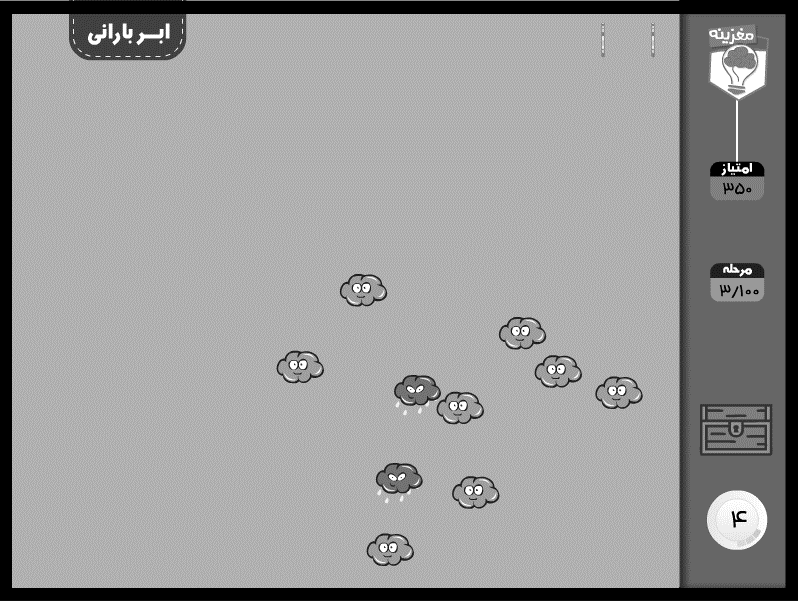
\includegraphics[scale=0.8]{Figures/cloudsGame.png}
\caption{\label{fig:cloudsGame}
بازی ابرهای باران‌زا
}
\end{figure}

برخی از ویژگی‌های بازی متناسب با نیازهای آزمایش تغییر داده شده است. به عنوان مثال در بازی اصلی به بازیکن به ازای هر انتخاب صحیح یک سکه تعلق می‌گیرد یا در برخی از مراحل تعدادی شیء به عنوان \mls{منحرف‌کننده} در صفحه نمایش داده می‌شوند. این موارد در بازی استفاده شده در این پژوهش، به علت حذف عوامل منحرف‌کننده، حذف شده‌اند. همچنین ترتیب مراحل و میزان سختی هر مرحله متناسب با نیازهای هر بخش تنظیم شده است.


\section{طراحی آزمایش اول}
نتایج آزمایشی که در این بخش طراحی شده است پیش‌نیاز آزمایش بخش بعدی است. این بخش دو هدف دارد. اول اینکه مجموعه‌ای از راهبرد‌های مورد استفاده‌ی افراد در بازی ابر باران‌زا استخراج شود و دوم اینکه یک رده‌بندی برای راهبرد‌های موجود ارائه شود. به این معنا که مشخص شود کدام راهبرد‌(ها) به صورت میانگین کارآیی بهتری داشتند. 

\subsection{ساختار آزمایش}
آزمایشی که در این بخش طراحی شد مشابه آزمایشی بود که برای انتخاب بازی انجام دادیم ولی چند تفاوت عمده داشت. اولین تفاوت مهم این بود که بازی را به ۷ بخش تقسیم کردیم. بخش اول مراحلی بودند که یک ابر بارانی داشتند، بخش دوم دو ابر بارانی داشتند و الی آخر. آزمون به این صورت است که ابتدا بازیکن یک بخش را کامل بازی می‌کند و سپس راهبرد‌های خود در آن بخش را یادداشت می‌کند. بازی از نظر زمانی محدود است. هر فرد ۱۰ دقیقه برای انجام بازی فرصت دارد. نحوه‌ی انتقال بین مراحل به این صورت است که اگر بازیکن تمام ابرهای باران‌زا را به درستی تشخیص دهد به مرحله‌ی بعدی می‌رود. اما اگر حتی یکی از آنها را اشتباه انتخاب کند در همان مرحله باقی می‌ماند. محدودیت تکرار هر مرحله ۲۰ بار است. یعنی اگر فردی بعد از ۲۰ بار تکرار یک مرحله نتواند آن را با موفقیت پشت سر بگذارد امتیازی از آن مرحله به او تعلق نخواهد گرفت. بازی در مجموع ۴۲ مرحله است. تعداد مراحل در هر بخش در جدول \ref{numOfLevelTable} نمایش داده شده است.

\begin{table}[]
\centering
\caption{تعداد مراحل هر بخش}
\label{numOfLevelTable}
\begin{tabular}{|c|c|}
\hline
\textbf{تعداد مراحل} & \textbf{شماره بخش} \\ \hline
۴                    & ۱                  \\ \hline
۵                    & ۲                  \\ \hline
۶                    & ۳                  \\ \hline
۶                    & ۴                  \\ \hline
۷                    & ۵                  \\ \hline
۷                    & ۶                  \\ \hline
۷                    & ۷                  \\ \hline
\end{tabular}
\end{table}


بین هر دو بخش توقفی وجود دارد تا بازیکن فرصت داشته باشد راهبرد‌های خود را بنویسد که در آن زمان بازی متوقف می‌شود. در نهایت پس از اتمام زمان از بازیکن تقاضا می‌شود پرسشنامه‌ی اطلاعات فردی را تکمیل کند. این پرسشنامه در بخش \ref{attachment1} پیوست شده است.
آزمون با استفاده از نرم‌افزار  \lr{adobe flash cs6}و با استفاده از زبان برنامه‌نویسی  \lr{action script 3} طراحی شد. برای اجرای آزمون از یک لپ تاپ (\lr{Lenovo ThinkPad E460}) استفاده شد و شرکت کننده‌ها با استفاده از نشانگر جواب خود را انتخاب می‌کردند.

\subsection{ثبت داده}
در این مرحله اطلاعات را با استفاده از دو ابزار مختلف ثبت می‌کنیم. ابزار اول استفاده از اطلاعات ثبت شده از نحوه‌ی بازی کردن آزمون‌دهنده است. به ازای هر مرحله این اطلاعات شامل مکان ابرهای بارانی و عادی، تعداد ابرهایی که به درستی انتخاب شدند، تعداد ابرهایی که به اشتباه انتخاب شدند، مکان نشانگر در هر لحظه و ویژگی‌های آن مرحله از بازی است.
ابزار دیگری که برای ثبت اطلاعات از آن استفاده کردیم یک دستگاه ردیاب چشم بود. (توضیح ویژگی‌های دستگاه) هدف استفاده از این دستگاه ثبت نقطه‌ی نگاه آزمون دهنده و تطبیق آن با راهبرد‌های گزارش شده توسط وی بود.

\subsection{شرکت‌کننده‌ها}
در این مرحله، آزمون به صورت یک مسابقه برگزار شد. مجموعا ۵۷ نفر در مسابقه شرکت کردند که از بین آنها اطلاعات ۴۶ نفر با توجه به پرسشنامه‌ها قابل استفاده بود. از میان این ۴۶ نفر ۱۴ نفر زن و ۳۲ نفر مرد بودند. میانگین سنی آنها ۲۳ سال با انحراف معیار ۴ بود. به عنوان جایزه به دو نفری که بیشترین امتیاز را کسب کردند یک حافظه جانبی با ظرفیت ۳۲ گیگابایت داده شد و به دو نفر نیز به قید قرعه یک حافظه جانبی با ظرفیت ۱۶ گیگابایت داده شد.

\subsection{نحوه محاسبه امتیاز هر بازیکن}
دو معیار برای محاسبه‌ی امتیاز اهمیت دارند. اولین معیار آخرین مرحله‌ای است که شرکت‌کننده موفق شده به آن برسد و معیار دوم میزان توقف وی در مراحل است. به عنوان مثال فردی که توانسته همه‌ی مراحل را با یک بار بازی کردن پشت سر بگذارد و تا مرحله‌ی ۳۰ جلو برود باید امتیاز بیشتری از فردی بگیرد که تا مرحله‌ی ۳۰ جلو رفته اما هر مرحله را ۲ بار انجام داده است.
علاوه بر این هزینه‌ی خطاها در مراحل بالاتر بیشتر است. به این معنی که فردی که مرحله‌ی ۱ را ۵ بار تکرار کرد امتیاز بیشتری می‌گیرد نسبت به فردی که مرحله‌ی ۲۰ را ۵ بار تکرار کرده است (با فرض اینکه بقیه‌ی مراحل را مشابه هم بازی کرده باشند).
با توجه به این موضوع معیار امتیاز دهی را به این صورت تعیین کردیم که شماره‌ی مرحله ضریب امتیاز آن مرحله باشد و تعداد تکرارهای هر مرحله از ۲۱ کم می‌شود و در ضریب آن مرحله ضرب می‌شود. در نهایت امتیاز همه‌ی مراحل با هم جمع می‌شوند. نحوه‌ی محاسبه‌ی امتیاز در رابطه‌ی \ref{eq:levelScore} نشان داده شده است.

\begin{equation}
\label{eq:levelScore}
	score = \sum_{level=1}^{lastLevelReached} level(21-numOfLevelRepeat)
\end{equation}


\section{نتایج بخش اول}
در بخش اول دو هدف اصلی را دنبال می‌کردیم. هدف اول جمع‌آوری مجموعه‌ای از راهبرد‌های مورد استفاده توسط افراد بود و هدف دوم طبقه‌بندی این راهبرد‌ها بر اساس میزان موثر بودن آنها بوده است. به منظور جمع‌آوری راهبردها از روش تحلیل محتوا استفاده شده است.  ابتدا تمامی پرسشنامه‌ها خوانده شدند و راهبردهایی که مشابه هم بودند استخراج و کدگزاری شدند. سپس مجددا تمامی پرسشنامه‌ها بررسی شدند و اطمینان حاصل شد که تمامی راهبرد‌های نوشته شده به حداقل یک راهبرد استخراج شده مرتبط می‌شود.

\subsection{راهبرد‌های استخراج شده}
در این بخش راهبرد‌های جمع‌آوری شده را  به دو دسته‌ی اصلی و فرعی تقسیم  کردیم. منظور از راهبردهای اصلی راهبرد‌هایی است که عمده‌ی عملکرد فرد تحت تاثیر آن قرار می‌گیرد و به تنهایی می‌تواند راهبرد فرد در طی آزمایش باشد. راهبردهای فرعی راهبردهایی هستند که فرد از آنها در کنار یک راهبرد اصلی استفاده می‌کند. در جدول \ref{StrategyList} لیست راهبرد‌های اصلی نمایش داده شده است.
\begin{table}[]
	\centering
	\caption{راهبرد‌های اصلی}
	\label{StrategyList}
	\begin{scriptsize}
	\begin{center}
	\renewcommand{\arraystretch}{2}
	\begin{tabular}{|c|c|r|}
		\hline
\textbf{شماره گروه} & \textbf{شماره راهبرد} & \multicolumn{1}{c|}{\textbf{توضیح راهبرد}} \\ \hline
		\multirow{4}{*}{۱} & 1 & دنبال کردن ابر با چشم \\ \cline{2-3} 
		& 2 & دنبال کردن ابر با استفاده از ماوس \\ \cline{2-3} 
		& 3 & دنبال کردن ابر با استفاده از انگشتان دست \\ \cline{2-3} 
		& 4 & سوئیچ کردن نگاه بین ابرها \\ \hline
		\multirow{5}{*}{۲} & 5 & نگاه کردن به مرکز صفحه یا مرکز ابرهای باران‌زا یا نگاه کلی به صفحه (نگاه کردن کل ابرها به صورت همزمان) \\ \cline{2-3} 
		& 6 & نگاه کردن به یک ابر باران‌زا در حالی که سایر ابرها در دامنه دید هستند \\ \cline{2-3} 
		& 7 & سوئیچ کردن نگاه بین مرکز دو دسته ابر باران‌زا \\ \cline{2-3} 
		& 8 & تصور کردن به صورت خط یا شکل هندسی \\ \cline{2-3} 
		& 9 & دنبال کردن برخی از ابرها با یک چشم و برخی دیگر با چشم دیگر \\ \hline
		\multirow{4}{*}{۳} & 10 & توجه بیشتر به ابرهای نواحی شلوغ \\ \cline{2-3} 
		& 11 & توجه بیشتر به ابرهایی که سرعت و دامنه حرکت بیشتری دارند \\ \cline{2-3} 
		& 12 & توجه بیشتر به نواحی که ابرهای باران‌زای بیشتری دارند \\ \cline{2-3} 
		& 13 & توجه بیشتر به ابرهایی که در یک جهت حرکت می‌کردند \\ \hline
	\end{tabular}
	\end{center}
	\end{scriptsize}
\end{table}

راهبرد‌های جدول \ref{StrategyList} که در یک دسته قرار گرفته‌اند ویژگی‌های مشابه دارند. این ویژگی‌ها در جدول \ref{mainStrategyGroups} نمایش داده شده‌اند. در نهایت دسته‌ها با یکدیگر مقایسه شده‌اند.

\begin{table}[]
\centering
\caption{ویژگی‌های مشترک هر دسته از راهبرد‌ها}
\label{mainStrategyGroups}
\begin{scriptsize}
\begin{center}
\renewcommand{\arraystretch}{2}
\begin{tabular}{|c|r|}
\hline
\textbf{شماره گروه} & \multicolumn{1}{c|}{\textbf{ویژگی مشترک}} \\ \hline
۱ & نقطه تمرکز چشم در هر لحظه روی یک ابر بارانی است \\ \hline
۲ & نقطه تمرکز چشم در هر لحظه روی هیچ کدام از ابرهای بارانی نیست \\ \hline
۳ & نقطه تمرکز چشم بعضی اوقات روی یکی از ابرها و بعضی اوقات در نقطه‌ای خارج از ابرهای بارانی است. \\ \hline
\end{tabular}
\end{center}
\end{scriptsize}
\end{table}
در جدول \ref{secondaryStrategies} لیست راهبرد‌های فرعی نمایش داده شده‌اند.

\begin{table}[]
\centering
\caption{راهبرد‌های فرعی}
\label{secondaryStrategies}
\begin{scriptsize}
\begin{center}
\renewcommand{\arraystretch}{2}
\begin{tabular}{|c|r|}
\hline
\textbf{شماره راهبرد} & \multicolumn{1}{c|}{\textbf{توضیح راهبرد}} \\ \hline
۱ & جدا کردن یک یا چند ابر و دنبال کردن آن با گوشه چشم (دامنه بینایی) یا ماوس \\ \hline
۲ & صرف نظر کردن از تعدادی از ابرها \\ \hline
۳ & پیش‌بینی حرکت برخی از ابرها \\ \hline
۴ & افزایش توجه هنگام کند شدن حرکت ابرها \\ \hline
۵ & ثبت یک تصویر ذهنی از مکان ابرها هنگامی که رنگشان تغییر می‌کند \\ \hline
۶ & تنگ‌تر کردن چشم \\ \hline
\end{tabular}
\end{center}
\end{scriptsize}
\end{table}


\subsection{روش محاسبه امتیاز هر راهبرد}
به منظور امتیازدهی به راهبرد‌ها ابتدا امتیاز هر  \mls{شرکت‌کننده} در هر بخش را محاسبه کردیم. روش محاسبه‌ی امتیاز در هر بخش مشابه روش محاسبه‌ی امتیاز کل هر شرکت‌کننده بود با این تفاوت که به جای اینکه تمامی مراحل در امتیاز دهی دخیل باشند تنها مراحل همان بخش در امتیازدهی دخیل بودند. با توجه به اینکه شماره مراحل بخش‌های آخر بیشتر از شماره مراحل بخش‌های اول بودند امتیاز مراحل آخر نیز از سطح بالاتری شروع می‌شدند. به عنوان مثال کسی که یک مرحله از بخش ۷ را انجام دهد امتیاز بیشتری از بخش ۷ می‌گیرد نسبت به کسی که یک مرحله از بخش ۲ را انجام می‌دهد. امتیاز هر مرحله با استفاده از رابطه‌ی \ref{levelScoreEq} محاسبه می‌شود.
\begin{equation}
\label{levelScoreEq}
	score(person = i, part = j) = \sum_{level = FirstLevel(j)}^{LastLevel(j)} level(21-numOfLevelRepeat(level, i))
\end{equation}

هدف نهایی این بخش این است که بفهمیم هر راهبرد در هر بخش به صورت میانگین چقدر امتیاز برای شرکت‌کننده‌گان کسب کرده است. راهبرد‌ی که موفق شده باشد میانگین امتیاز بالاتری کسب کند راهبرد برنده در آن بخش است. به همین منظور پس از اینکه امتیاز هر بخش محاسبه شد با استفاده از آن، امتیاز هر راهبرد را محاسبه می‌کنیم. برای این کار از رابطه‌ی \ref{StrategyScoreEq} استفاده می‌کنیم. در این رابطه n  تعداد کل افراد شرکت‌کننده در آزمایش است. 

\begin{equation}
\label{UseStrategyEq}
useStrategy(person = i, strategy = k, part = j) =\begin{cases}
    1 ,& \text{\lr{if person i used strategy k in part j}} \\
    0 , & \text{otherwise}
    \end{cases}
\end{equation}


\begin{equation}
count(strategy = k, part = j) = \sum_{i=1}^{n} useStrategy(i, k, j)
\end{equation}

\begin{equation}
\label{StrategyScoreEq}
	score(strategy = k, part = j) = \frac{1}{count(k, j)} \sum_{i=1}^{n} score(person = i, part = j) useStrategy(i, k, j)
\end{equation}

امتیاز هر راهبرد بر اساس این روابط میانگین امتیازهایی است که هر فرد با استفاده از این راهبرد به دست آورده است.

\subsection{تحلیل امتیاز هر بخش}
برای تحلیل امتیاز هر گروه راهبرد در هر بخش ابتدا باید توزیع این داده‌ها را بررسی کنیم. اگر توزیع داده‌ها نزدیک به نرمال باشد می‌توانیم از آزمون t یا \mls{آنالیز واریانس} استفاده کنیم. در غیر این صورت باید از آزمون‌های غیر پارامتری مانند \mls{ویلکاکسون} و \mls{کروسکال-والیس} استفاده کنیم. در شکل 
در شکل \ref{fig:extractStrategyPartsHist} می‌توانیم میانگین هر گروه راهبرد در بخش‌های مختلف را ببینیم.

\begin{figure}
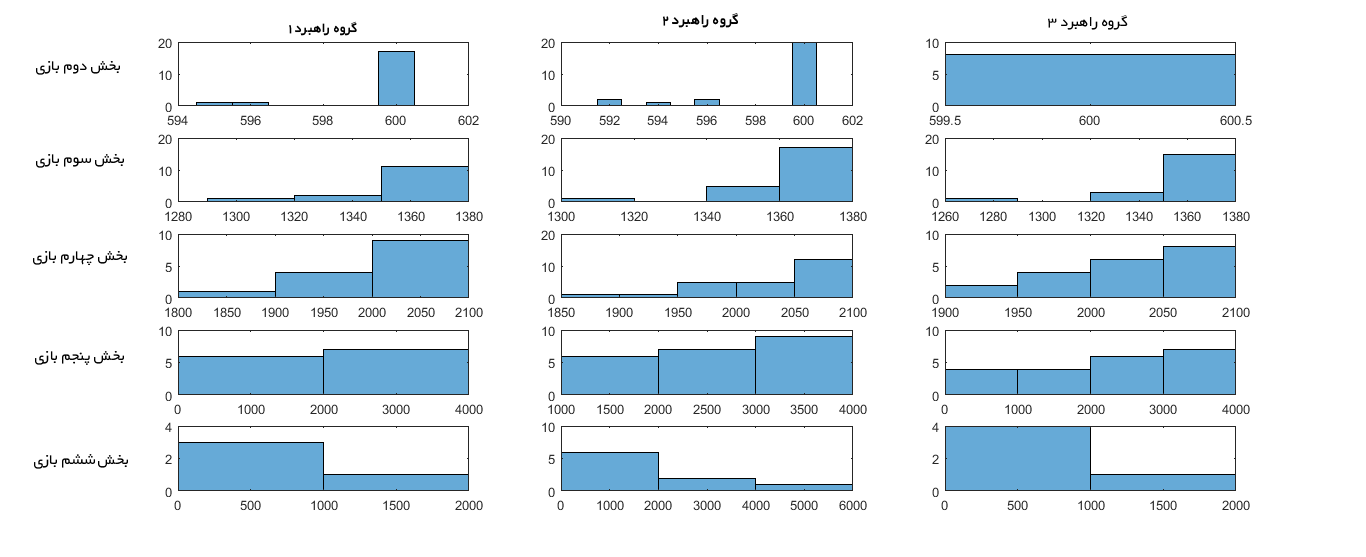
\includegraphics[width=1\textwidth, center]{Figures/extractStrategyPartsHist.png}
\caption{\label{fig:extractStrategyPartsHist}
هیستوگرام امتیاز راهبردهای مختلف در بخش‌های ۲ تا ۶
}
\end{figure}

با توجه به شکل \ref{fig:extractStrategyPartsHist} می‌بینیم که توزیع داده‌ها از توزیع نرمال خیلی فاصله دارد در نتیجه نمی‌توانیم از آزمون t  یا آنالیز واریانس استفاده کنیم. به همین دلیل در این بخش از آزمون کروسکال-والیس استفاده خواهیم کرد. در این آزمون حداقل سطح معناداری برابر با $\alpha = 0.05$ در نظر گرفته شده است.

در شکل \ref{fig:part2-6MedianOfScores} میانه‌ی گروه‌های مختلف راهبردها در بخش‌های مختلف نمایش داده شده است. همانطور که مشخص است میانه‌ی گروه راهبرد ۲ در تمامی بخش‌ها بیشتر از دو گروه راهبرد دیگر است.
\begin{figure}
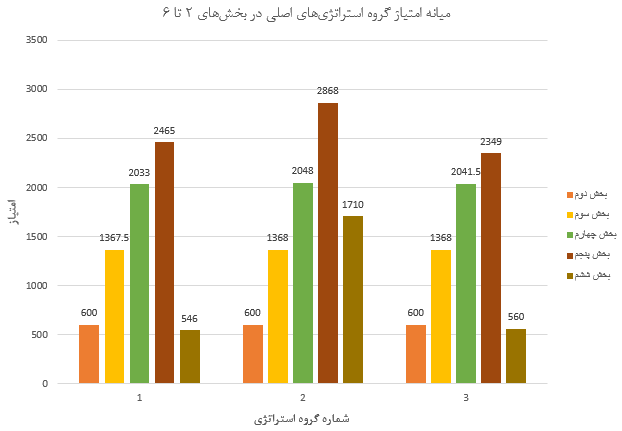
\includegraphics[width=1\textwidth, center]{Figures/part2-6MedianOfScores.png}
\caption{\label{fig:part2-6MedianOfScores}
میانه‌ی گروه‌های راهبرد ۱-۳ در بخش‌های ۲-۶
}
\end{figure}

در جدول \ref{tbl:kruskalWallisRes} مقادیر p-value هر بخش پس از انجام آزمون کروسکال-والیس نمایش داده شده است.

\begin{table}[]
\begin{scriptsize}
\begin{center}
\centering
\caption{مقادیر p-value مربوط به هر بخش پس از انجام آزمون کروسکال-والیس}
\label{tbl:kruskalWallisRes}
\renewcommand{\arraystretch}{2}
\begin{tabular}{|c|c|}
\hline
\textbf{شماره بخش} & p-value\\ \hline
\textbf{\begin{tabular}[c]{@{}c@{}}بخش ۲\end{tabular}} & ۰/۳۰\\ \hline
\textbf{\begin{tabular}[c]{@{}c@{}}بخش ۳\end{tabular}} & ۰/۶۷\\ \hline
\textbf{\begin{tabular}[c]{@{}c@{}}بخش ۴\end{tabular}} & ۰/۴۹\\ \hline
\textbf{\begin{tabular}[c]{@{}c@{}}بخش ۵\end{tabular}} & ۰/۲۰\\ \hline
\textbf{\begin{tabular}[c]{@{}c@{}}بخش ۶\end{tabular}} & ۰/۰۴\\ \hline
\end{tabular}
\end{center}
\end{scriptsize}
\end{table}

همانطور که مشخص است مقدار p-value تنها در بخش ۶ کمتر از $\alpha$ است و به همین دلیل تنها در بخش ۶ می‌توانیم بگوییم میانه امتیاز در بخش‌های مختلف تفاوت معناداری با یکدیگر دارند. در جدول \ref{tbl:coxonpart6Str1to3} سه گروه راهبرد بخش ۶ را به صورت جداگانه با استفاده از آزمون ویلکاکسون با هم مقایسه کرده‌ایم. همانطور که مشخص است نتایج نشان می‌دهد گروه راهبرد ۲ به طرز معناداری از گروه راهبرد ۳ بهتر عمل کرده است. البته در تمام بخش‌ها گروه راهبرد ۲ میانه امتیازی نسبت به دو گروه دیگر بیشتر بوده ولی در مقایسه با گروه راهبرد ۱ مقدار آن معنادار نمی‌باشد.

\begin{table}[]
\begin{scriptsize}
\begin{center}
\centering
\caption{مقادیر p-value مربوط به راهبردهای مختلف بخش ۶}
\label{tbl:coxonpart6Str1to3}
\renewcommand{\arraystretch}{2}
\begin{tabular}{|c|c|}
\hline
\textbf & p-value\\ \hline
\textbf{\begin{tabular}[c]{@{}c@{}}گروه راهبرد ۱ در مقایسه با ۲\end{tabular}} & ۰/۰۶\\ \hline
\textbf{\begin{tabular}[c]{@{}c@{}}گروه راهبرد ۱ در مقایسه با ۳\end{tabular}} & ۱\\ \hline
\textbf{\begin{tabular}[c]{@{}c@{}}گروه راهبرد ۲ در مقایسه با ۳\end{tabular}} & ۰/۰۴\\ \hline
\end{tabular}
\end{center}
\end{scriptsize}
\end{table}

برای تحلیل راهبردهای فرعی نیز از روش مشابهی استفاده کردیم ولی به علت محدود بودن داده‌های مربوط به راهبردهای فرعی هیچ تفاوت معناداری بین آنها پیدا نشد. در هر بخش برخی از این راهبردها نمره‌ی بیشتری کسب کرده‌اند ولی هیچ کدام از آنها نسبت به دیگری از لحاظ آماری برتری نداشتند.


\subsection{راهبردهای منتخب برای آزمایش دوم}

نتایج به دست آمده از بخش قبل نشان می‌دهد که گروه دوم راهبردها به نسبت گروه ۱ و ۳ میانه امتیاز بیشتری در همه‌ی بخش‌ها دارند. اما از نظر آماری تنها در بخش ششم گروه راهبرد ۲ تفاوت معناداری با سایر گروه‌های راهبرد پیدا کرده است. با توجه به اینکه اکثر افراد تا بخش ۴ به راحتی جلو می‌آیند و از این نقطه به بعد است که با مشکل مواجه می‌شوند راهبرد موثر در بخش ۴ و ۵ و ۶ اهمیت بیشتری پیدا می‌کند. با توجه به اینکه میانه‌ی نمره‌ی گروه راهبرد ۲ در تمام بخش‌ها بیشتر از سایر گروه‌ها است و در بخش ۶ تفاوت معناداری با سایر گروه‌ها دارد این گروه راهبرد برای آموزش در بخش بعدی انتخاب می‌شود.

\subsection{مشکلات موجود در آزمایش اول}

مشکلاتی در آزمایش اول وجود داشتند که در این بخش به آنها می‌پردازیم. اولین موضوع کم بودن تعداد افرادی بود که در آزمایش شرکت کردند. به خصوص با توجه به طیف گسترده‌ی راهبردها و روش‌های مختلفی که افراد حین بازی کردن از آن استفاده می‌کردند کم بودن افراد باعث شد در برخی از موارد اطلاعات کافی برای تحلیل نداشته باشیم. به عنوان مثال در مورد راهبردهای فرعی کمبود داده باعث شد نتوانیم تحلیل جامعی ارائه دهیم. پیشنهادی که برای آینده ارائه می‌شود این است که این تست به صورت \mls{برخط} برگزار شود و افراد راهبردهای مورد استفاده‌ی خود را به صورت گزینه‌ای گزارش کنند تا امکان جمع‌آوری اطلاعات در تعداد بالا ایجاد شود.

مشکل دیگر کوتاه بودن مدت زمان آزمایش بود. افراد ۱۰ دقیقه فرصت داشتند که بازی کنند و راهبردهای خود را بنویسند. این موضوع باعث می‌شد فرصت اندکی برای حرفه‌ای شدن در بازی و رسیدن به راهبردهای موثر وجود داشته باشد. پیشنهاد می‌شود در پژوهش‌های آتی از یک دوره‌ی تمرینی استفاده شود. به این صورت که افراد حدودا یک ماه فرصت داشته باشند که بازی کنند و در طی این مدت راهبردهای خود را به مرور به روز کنند.

\chapter{آزمایش دوم - انتقال راهبرد}
\label{chapter:PartTwoTransfer}
\thispagestyle{plain}

\section{مقدمه}
در این بخش هدف اصلی بررسی تاثیر انتقال راهبرد بر عملکرد بازیکن است. به این منظور از نتایج به دست آمده در بخش قبل استفاده می‌کنیم و راهبرد انتخاب شده را با استفاده از دو روش به بازیکن منتقل کنیم. علاوه بر این، موضوع دیگری که در این بخش مورد بررسی قرار می‌گیرد رابطه‌ی میان مدل تصمیم‌گیری بازیکن (مدل محور یا مدل آزاد بودن) و میزان یادگیری راهبرد است.

\section{طراحی آزمایش دوم}
\subsection{ساختار آزمایش اصلی} \label{partTwoMainTest}

این آزمایش از ۳ بخش تشکیل شده است.
\subsubsection{بخش اول}
در بخش اول افراد در \mls{آزمون دو مرحله‌ای دا} که در \cite{daw2011ModelBased} توضیح داده شده است، شرکت کردند. این آزمون از دو بخش تمرینی و اصلی تشکیل شده است. بخش تمرینی شامل ۴۰ دور و بخش اصلی شامل ۲۰۰ دور است. در هر دور افراد ابتدا تصویر دو هواپیما را مشاهده می‌کنند سپس ۲ ثانیه فرصت دارند که با استفاده از کلید f یا j یکی از این دو تصویر را انتخاب کنند. پس از انتخاب کردن یکی از این دو تصویر به یکی از دو جنگل موجود راهنمایی می‌شوند. دو تصویر از جنگل انتخاب شده نمایش داده می‌شود. مجددا بازیکن باید با استفاده از کلید f  یا j یکی از دو تصویر را انتخاب کند. پس از انتخاب تصویر به او نمایش داده می‌شود که در آن جنگل گنج وجود دارد یا خیر. اگر گنج وجود داشته باشد امتیاز می‌گیرد و اگر وجود نداشته باشد امتیازی نمی‌گیرد.
احتمال رفتن به هر جنگل پس از انتخاب هر هواپیما در شکل \ref{fig:plainJungleProb} مشخص شده است. با انتخاب هواپیمای سفید با احتمال ۳۰ درصد به جنگل سمت راست و با احتمال ۷۰ درصد به جنگل سمت چپ می‌رود و با انتخاب هواپیمای نارنجی احتمال‌ها برعکس می‌شوند.
احتمال وجود داشتن گنج در هر جنگل از توزیع \mls{قدم زدن تصادفی} پیروی می‌کند. بنابراین این احتمال در هر جنگل در حال تغییر است و بازیکن در حین بازی با امتحان کردن حالت‌های مختلف باید تلاش کند بیشترین امتیاز را کسب کند.
\begin{figure}
\centering
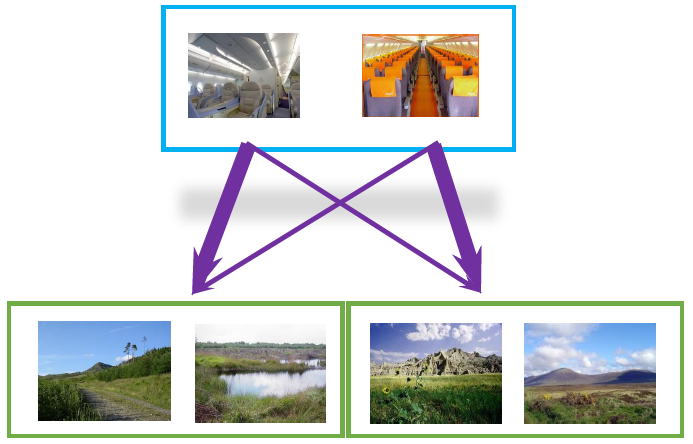
\includegraphics[scale=0.8]{Figures/plainJungleProb.png}
\caption{\label{fig:plainJungleProb}
احتمال منتقل شدن از هر هواپیما به هر جنگل
}
\end{figure}

\subsubsection{بخش دوم}

در بخش دوم، از بازی «ابر باران‌زا» که در آزمایش اول استفاده شده بود، استفاده می‌شود منتها ساختار آزمایش متفاوت است. در این بخش آزمایش به این صورت طراحی شده است که ابتدا ۴ مرحله‌ی آزمایشی اجرا می‌شود که ۱ یا ۲ ابر باران‌زا دارند. این چهار مرحله به منظور آشنایی بازیکن با ساختار و نحوه‌ی انجام بازی قرار داده شده‌اند. سپس بازی اصلی شروع می‌شود. بازی اصلی شامل ۵ بخش است. بخش اول شامل ۳ ابر باران‌زا است (به همین دلیل بخش ۳ نامیده شده است) و به ترتیب بخش‌های بعدی شامل ۴و ۵ و ۶و ۷ ابر باران‌زا هستند. بر خلاف آزمایش اول که محدودیت زمانی داشت در این آزمایش محدودیت زمانی نداریم. ساختار بازی به این صورت است که هر بخش شامل ۱۰ مرحله است. در هر مرحله اگر بازیکن موفق شود تمامی ابرها را به درستی تشخیص دهد امتیاز آن مرحله را کامل دریافت می‌کند اما اگر حتی یکی از ابرها را درست تشخیص ندهد هیچ امتیازی از آن مرحله کسب نخواهد کرد. در انتهای هر بخش درصد مراحلی که با موفقیت گذرانده محاسبه می‌شود. برای هر بخش یک حد نصاب در نظر گرفته شده است که اگر بازیکن بتواند حد نصاب را کسب کند می‌تواند وارد بخش بعدی شود. اگر موفق نشود می‌تواند تا زمانی که بخواهد آن بخش را مجددا بازی کند تا جایی که به این نتیجه برسد که نمی‌تواند این درصد را بهبود ببخشد و انتخاب می‌کند بازی تمام شود. حد نصاب بخش‌های مختلف در جدول \ref{tbl:quorum} نمایش داده شده است. 

\begin{table}[]
\begin{scriptsize}
\begin{center}
\centering
\caption{حد نصاب بخش‌های مختلف برای رفتن به بخش بعدی در آزمایش دوم}
\label{tbl:quorum}
\renewcommand{\arraystretch}{2}
\begin{tabular}{|c|c|}
\hline
\textbf{شماره بخش}& \textbf{حد نصاب}\\ \hline
\textbf{\begin{tabular}[c]{@{}c@{}}بخش ۳ به ۴\end{tabular}} & موفقیت در حداقل ۸۰ درصد مراحل\\ \hline
\textbf{\begin{tabular}[c]{@{}c@{}}بخش ۴ به ۵\end{tabular}} & موفقیت در حداقل ۶۰ درصد مراحل\\ \hline
\textbf{\begin{tabular}[c]{@{}c@{}}بخش ۵ به ۶\end{tabular}} & موفقیت در حداقل ۵۰ درصد مراحل\\ \hline
\textbf{\begin{tabular}[c]{@{}c@{}}بخش ۶ به ۷\end{tabular}} & موفقیت در حداقل ۵۰ درصد مراحل\\ \hline
\end{tabular}
\end{center}
\end{scriptsize}
\end{table}

حدنصاب‌های به دست آمده با استفاده از اطلاعات جمع‌آوری شده در آزمایش اول استخراج شده‌اند. به این صورت که درصد مراحلی که هر بازیکن توانسته در هر بخش به صورت موفقیت آمیز انجام بدهد محاسبه شده و سپس بین تمامی افراد میانگین گرفته شده است. پس از اتمام هر بخش از بازیکن خواسته می‌شود راهبرد مورد استفاده‌ی خود را یادداشت کند.  

\subsubsection{بخش سوم} \label{partTwoMainTest:three}

پس از اتمام دور اول بازی، راهبرد انتخاب شده در آزمایش اول به صورت کلامی به بازیکن آموزش داده می‌شود. در این راهبرد از بازیکن خواسته می‌شود در حین انجام آزمایش به مرکز ابرهای باران‌زا نگاه کند در حالی که ابرها در دامنه‌ی دیدش هستند. یا به بیان دیگر یک چند ضلعی فرضی در نظر بگیرد و مرکز آن را نگاه کند. علاوه بر آموزش کلامی یک راهنما نیز در بازی قرار داده شده است تا بازیکن با استفاده از آن، راهبرد جدید را بیاموزد. این راهنما به این صورت عمل می‌کند که در ۵ مرحله‌ی ابتدایی هر بخش بازیکن به صورت اختیاری امکان استفاده از راهنما را خواهد داشت. اگر گزینه‌ی استفاده از راهنما را انتخاب کند نقطه‌ی مرکزی ابرهای باران‌زا و \mls{بدنه‌ی محدب} آنها نمایش داده می‌شود. در حین کند شدن حرکت ابرها راهنما نیز کمرنگ می‌شود تا نهایتا حذف شود. از بازیکن‌ها خواسته می‌شود پس از اتمام هر بخش میزان استفاده‌ی خود از راهبرد آموزش داده شده را توسط عددی بین ۱ تا ۵ مشخص کنند. ۱ به این معنا است که در هیچ کدام از مراحل نتوانسته‌اند از راهبرد استفاده کنند و ۵ به این معنا است که در تمامی مراحل موفق به استفاده از آن شده‌اند. در این بخش نیز مانند بخش دوم بازی، بازیکن می‌تواند هر بخش را مطابق تشخیص خود تکرار کند.

\subsubsection{پس از اتمام}

پس از اتمام آزمایش به منظور درک دقیق‌تر راهبردهای استفاده شده بازیکن، لیستی از راهبردهای جمع‌آوری شده به او ارائه می‌شود و از او خواسته می‌شود راهبردهایی که خود نوشته است با راهبردهای این لیست تطبیق بدهد. در نهایت با پر کردن فرم اطلاعات فردی آزمایش به پایان می‌رسد. پانزده هزار تومان بابت شرکت کردن در آزمایش و پانزده هزار تومان به نسبت عملکرد هر فرد به او داده می‌شود.
طراحی ساختار آزمایش به شکل کنونی سه دلیل اصلی دارد. اول اینکه محدودیت زمانی باعث کاهش کارآیی فرد نشود. دوم اینکه می‌خواهیم بازیکن به بهترین عملکرد خود برسد. در واقع کمبود تمرین باعث محدود شدن کارآیی‌اش نشود. دلیل سوم که در ادامه‌ی دلیل دوم است این است که میخواهیم فرد به مرحله‌ای برسد که با تمرین بیشتر عملکردش بهبود پیدا نکند. در واقع به نقطه‌ای برسد که حد توانمندی فردی اوست. دلیل این است که می‌خواهیم احتمال بهبود عملکرد با تمرین بیشتر، کاهش پیدا کند. بازیکن به نقطه‌ای برسد که خودش نتواند با تمرین بیشتر بهبود قابل توجهی پیدا کند و سپس بررسی کنیم آیا در این مرحله آموزش راهبرد موثر واقع می‌شود یا خیر.

\subsection{گروه کنترلی اول}

در راستای مقایسه‌ی نتایج به دست آمده از آزمایش اصلی، یک آزمایش دیگر انجام شد که در آن راهبرد موثر به افراد آموزش داده نمی‌شود. ساختار آزمایش دو تفاوت با آزمایش اصلی دارد. اول اینکه آزمون مدل محور یا مدل آزاد بودن یادگیری فرد حذف شد و دوم اینکه آموزش راهبرد انجام نمی‌شود. سایر بخش‌های آزمایش مشابه آزمایش اصلی است.

\subsection{گروه کنترلی دوم}

موضوعی که باعث نیاز به گروه کنترلی دوم می‌شود این است که ممکن است گزارش دادن راهبرد روی عملکرد افراد تاثیر بگذارد. بنابراین نیاز به آزمایش دیگری داریم که افراد در آن درگیر گزارش راهبرد نشوند. این آزمایش به این صورت است که افراد دو بار بازی «ابرهای باران‌زا» را انجام می‌دهند بدون اینکه هیچ راهبردی گزارش کنند و در نهایت فرم اطلاعات فردی را تکمیل می‌کنند.

\subsection{شرکت‌کننده‌ها}

در آزمایش اصلی ۲۲ نفر شرکت کردند که ۷ نفر آنها زن و ۱۵ نفر مرد هستند. میانگین سنی آنها ۲۴ سال با انحراف معیار ۳ است. در آزمایش کنترلی اول ۲۰ نفر شرکت کردند که ۵ نفر آنها زن و ۱۵ نفر مرد هستند. میانگین سنی آنها ۲۶ سال با انحراف معیار ۲ است. در آزمایش کنترلی دوم ۱۸ نفر شرکت کردند که ۵ نفر آنها زن و ۱۳ نفر آنها مرد هستند. میانگین سنی آنها ۲۳ سال با انحراف معیار ۲ است.

\section{نتایج بخش دوم}

\subsection{مولفه‌های استخراج شده از داده‌ها}
در این بخش مولفه‌های استخراج شده از داده‌های به دست آمده از بازی‌ها را بررسی می‌کنیم و هر کدام را جداگانه تعریف می‌کنیم.
\subsubsection{مولفه‌های مربوط به مدل محور یا مدل آزاد بودن}

آزمون دا چندین مولفه را معرفی می‌کند. ما در این پژوهش از دو مولفه‌ی اصلی استفاده می‌کنیم: w و $\beta$. مولفه w عددی بین صفر و یک است و نشان‌دهنده‌ی میزان مدل محور بودن فرد است. هرچقدر w نزدیک‌تر به صفر باشد به این معنا است که فرد بیشتر مدل آزاد است و هر چقدر نزدیک به یک باشد به معنای مدل محور بودن فرد است. $\beta$ مولفه‌ی \mls{دمای معکوس} است. هرچه این مولفه مقدار کمتری داشته باشد به این معناست که فرد تمایل بیشتری به امتحان کردن انتخاب‌های جدید دارد و هرچه مقدار آن بیشتر باشد به این معناست که فرد تمایل بیشتری به ادامه‌ی انتخاب‌های پیشین خود دارد. در ادامه ارتباط این دو مولفه را با میزان استفاده‌ی بازیکن‌ها از راهبردها بررسی خواهیم کرد. 


\subsubsection{مولفه‌ی مربوط به میزان پیشرفت بازیکن}
همانطور که در بخش \ref{partTwoMainTest} مشخص شد بازی ۵ بخش اصلی دارد که هر کدام شامل ۱۰ مرحله هستند. بازیکن‌ها دو دور بازی می‌کنند. برای محاسبه‌ی درصد موفقیت فرد در هر بار بازی کردن از رابطه‌ی \ref{eq:partScoreEq} استفاده می‌کنیم. در این رابطه درصد وزن‌دار امتیاز کسب شده از بازی محاسبه می‌شود. به این صورت که بیشترین امتیازی که یک فرد می‌تواند از هر ۵ بخش کسب کند ۲۵۰ امتیاز است (در صورتی که تمامی مراحل تمامی بخش‌ها را با موفقیت انجام دهد) و امتیازی که کسب کرده حاصل جمع وزن‌دار امتیازش در هر بخش است. ضریب امتیاز هر بخش شماره‌ی همان بخش است. به این معنا که ۱ امتیاز بیشتر در بخش هفتم ارزش بیشتری از ۱ امتیاز بیشتر بخش سوم دارد. حاصل تقسیم این دو عدد درصد موفقیت فرد را مشخص می‌کند.

\begin{equation}
\label{eq:partScoreEq}
	gameScore = \frac{\sum_{i=3}^{7} numOfWonLevels(i)*i }{250}
\end{equation}

برای محاسبه‌ی پیشرفت بازیکن ابتدا درصد موفقیتش در هر دور از بازی را محاسبه می‌کنیم. سپس درصد پیشرفت وی را با استفاده از رابطه‌ی \ref{eq:improveEq} محاسبه می‌کنیم. این درصد در آزمایش‌های اصلی و کنترلی به همین شکل محاسبه شده است.

\begin{equation}
\label{eq:improveEq}
	scoreChangePercent(score1, score2) = \frac{score2 - score1}{score1}*100
\end{equation}

\subsubsection{مولفه مربوط به میزان استفاده از راهبرد}

همان‌طور که در بخش \ref{partTwoMainTest:three} گفته شد بازیکن‌ها میزان استفاده‌ی خود از راهبرد در هر بخش را توسط عددی بین ۱ تا ۵ گزارش می‌کنند. برای محاسبه‌ی میزان استفاده‌ی هر بازیکن از راهبردها می‌خواهیم درصد این استفاده را محاسبه کنیم. برای این کار از رابطه‌ی \ref{eq:strategyUsePercent} استفاده می‌کنیم. در این رابطه lastPart آخرین بخشی است که بازیکن موفق شده به آن برسد.
\begin{equation}
\label{eq:strategyUsePercent}
strategyUsePercent = \frac{\sum_{i=3}^{lastPart} useScore(i)}{lastPart*5}
\end{equation}

بنابراین هرچقدر بازیکن بیشتر موفق شده باشد در بخش‌هایی که بازی کرده از راهبرد استفاده کند این عدد نزدیک‌تر به ۱ خواهد بود.

\subsubsection{مولفه‌ی مربوط به زمان پاسخگویی}
علاوه بر میزان پیشرف بازیکن زمان پاسخگویی وی نیز می‌تواند حامل اطلاعات ارزشمندی باشد. به این منظور قصد داریم تغییرات مربوط به زمان پاسخگویی وی از دور اول بازی به دور دوم را بررسی کنیم. برای رسیدن به این هدف نیاز داریم برای هر دور از بازی میانگین زمان پاسخگویی را محاسبه کنیم. زمان پاسخگویی هر مرحله اختلاف بین زمان انتخاب آخرین ابر و اولین ابر است. بنابراین زمان پاسخگویی هر مرحله معلوم است. برای به دست آوردن زمان پاسخگویی یک دور از بازی از زمان پاسخگویی تمام مراحلی که بازیکن بازی کرده است میانگین می‌گیریم. بنابراین برای هر دور از بازی یک عدد به عنوان میانگین زمان پاسخگویی خواهیم داشت. با استفاده از رابطه‌ی \ref{eq:responseTimeDiffPercent} درصد تغییرات این میانگین را محاسبه می‌کنیم.

\begin{equation}
\label{eq:responseTimeDiffPercent}
	responseTimeChangePercent(t1, t2) = \frac{t2 - t1}{t1}*100
\end{equation}

\subsection{تحلیل همبستگی}
در این بخش قصد داریم میزان همبستگی بین مولفه‌های مختلف را بررسی کنیم. برای این کار از روش ضریب همبستگی  \mls{پیرسون} استفاده می‌کنیم.
\subsubsection{تحلیل همبستگی بین پیشرفت بازیکن و استفاده از راهبرد}

به منظور بررسی میزان همبستگی بین دو مولفه ابتدا \mls{نمودار نقطه‌ای} آنها را رسم می‌کنیم. این نمودار در شکل \ref{fig:impv1strUseScatter} نمایش داده شده است.

\begin{figure}
\centering
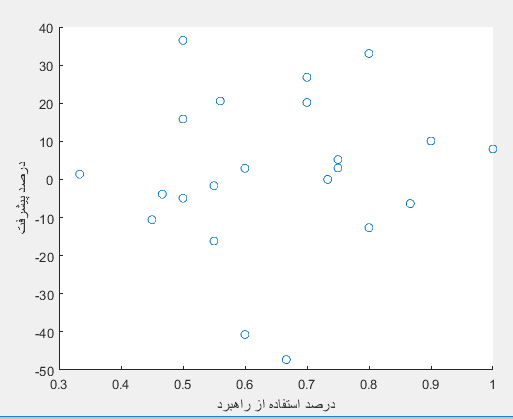
\includegraphics[scale=0.8]{Figures/impv1strUseScatter.png}
\caption{\label{fig:impv1strUseScatter}
نمودار نقطه‌ای پیشرفت بازیکن در برابر میزان استفاده‌ی وی از راهبرد
}
\end{figure}

سپس با استفاده از روش پیرسون ضریب همبستگی را حساب می‌کنیم. نتیجه‌ی به دست آمده نشان میدهد ضریب همبستگی برابر با ۰/۰۹ است و عدد p-value برابر با ۰/۶ است. این نتایج نشان می‌دهد این دو مولفه همبستگی معناداری با هم ندارند.

\subsubsection{تحلیل همبستگی بین استفاده از راهبرد و مولفه w }

مولفه‌ی w نشان می‌دهد بازیکن چه مقدار مدل محور است. هرچقدر این مولفه نزدیکتر به یک باشد به این معنا است که بازیکن بیشتر مدل محور است. مشابه بخش قبل از روش پیرسون برای محاسبه‌ی ضریب همبستگی استفاده می‌کنیم. نمودار نقطه‌ای این دو مولفه در شکل \ref{fig:stUsewScatter} نمایش داده شده است.

\begin{figure}
\centering
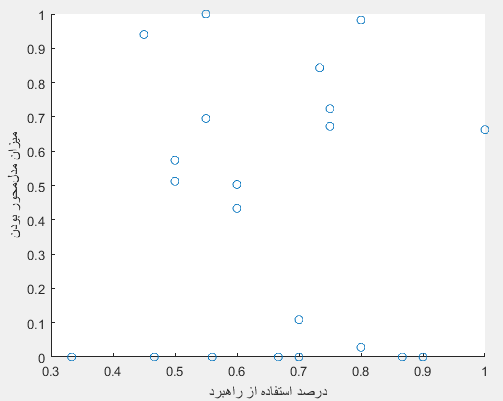
\includegraphics[scale=0.8]{Figures/stUsewScatter.png}
\caption{\label{fig:stUsewScatter}
نمودار نقطه‌ای مولفه‌ی w هر بازیکن در برابر میزان استفاده‌ی وی از راهبرد
}
\end{figure}

در این حالت ضریب همبستگی پیرسون برابر با ۰/۰۱- و عدد p-value برابر با ۰/۹ است که نشان می‌دهد این دو مولفه همبستگی معناداری با هم ندارند.

با توجه به نمودار \ref{fig:stUsewScatter} می‌توانیم مشاهده کنیم در تعداد زیادی از نقاط مقدار w بسیار نزدیک به صفر است. انتظار داریم افرادی که در آزمون دا نمره‌ای نزدیک به صفر می‌گیرند افرادی باشند که مدل آزاد هستند ولی حالت دیگری که ممکن است اتفاق بیافتد این است که مولفه w افرادی که از یادگیری تقویتی استفاده نکرده‌اند یا روش انجام دادن آزمون را به درستی متوجه نشده‌اند نیز نزدیک به صفر می‌شود. بنابراین تحلیل همبستگی را یک بار دیگر بعد از حذف داده‌هایی که w آنها صفر است تکرار می‌کنیم. نمودار نقطه‌ای نتیجه‌ی به دست آمده در شکل \ref{fig:stUsewScatterNoZero} نمایش داده شده است. در این حالت ضریب همبستگی برابر با ۰/۱۴- و عدد p-value برابر با ۰/۶ است که نشان می‌دهد در این حالت نیز همبستگی معناداری بین دو مولفه وجود ندارد.

\begin{figure}
\centering
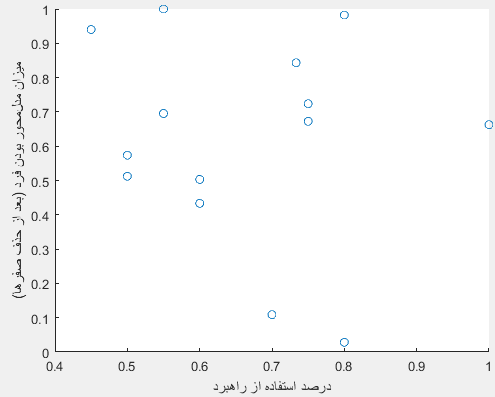
\includegraphics[scale=0.8]{Figures/stUsewScatterNoZero.png}
\caption{\label{fig:stUsewScatterNoZero}
نمودار نقطه‌ای مولفه‌ی w هر بازیکن در برابر میزان استفاده‌ی وی از راهبرد بعد از حذف w های صفر
}
\end{figure}

\subsubsection{تحلیل همبستگی بین استفاده از راهبرد و مولفه $\beta$}

مولفه‌ی $\beta$ معادل دمای معکوس است. هرچه دما بیشتر باشد $\beta$ کمتر است و به این معنا است که تمایل بازیکن به انتخاب گزینه‌های جدید و کاوش کردن محیط بیشتر است. هرچه دما کمتر باشد $\beta$ بیشتر است و به این معنا است که تمایل بازیکن به حفظ انتخاب‌های قبلی خود بیشتر است. می‌خواهیم میزان همبستگی $\beta$ با میزان استفاده از راهبرد را بسنجیم. در شکل \ref{fig:betaStUseScatter} نمودار نقطه‌ای این دو مولفه نمایش داده شده است. ضریب همبستگی پیرسون در این حالت برابر با ۰/۰۴ و عدد p-value برابر با ۰/۸۴ است که نشان می‌دهد این دو مولفه همبستگی معناداری با هم ندارند.

\begin{figure}
\centering
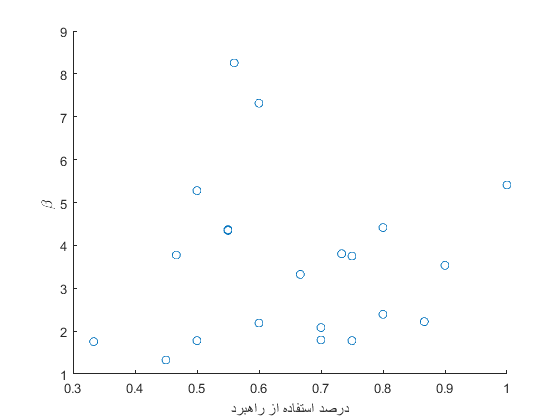
\includegraphics[scale=0.8]{Figures/betaStUseScatter.png}
\caption{\label{fig:betaStUseScatter}
نمودار نقطه‌ای مولفه $\beta$ هر بازیکن در برابر میزان استفاده‌ی وی از راهبرد
}
\end{figure}

\subsubsection{تحلیل همبستگی بین استفاده از راهبرد و تغییرات میانگین زمان پاسخگویی}

برای تحلیل این قسمت میانگین زمان پاسخگویی را به دو بخش تقسیم کردیم. افرادی که میانگین زمان پاسخگویی‌شان کاهش پیدا کرده و در نتیجه تغییرات میانگین زمان پاسخگویی‌شان منفی است و افرادی که میانگین زمان پاسخگویی‌شان افزایش پیدا کرده و در نتیجه تغییرات میانگین زمان پاسخگویی‌شان مثبت است. از بین ۲۲ نفری که در آزمایش شرکت کردند ۱۷ نفر کاهش میانگین زمان پاسخگویی و ۵ نفر افزایش میانگین زمان پاسخگویی داشتند. با توجه به اینکه تعداد افرادی که افزایش میانگین زمان پاسخگویی داشتند خیلی کم است نتایج به دست آمده از تحلیل همبستگی آنها معنادار نیست. نمودار نقطه‌ای افرادی که میانگین زمان پاسخ‌شان منفی است در شکل \ref{fig:stUseDtScatter} نمایش داده شده است. در این حالت ضریب همبستگی معادل ۰/۴۸ و عدد p-value برابر با ۰/۰۴۹ است. این مقادیر نشان می‌دهند این دو مولفه با هم همبستگی معناداری دارند.

\begin{figure}
\centering
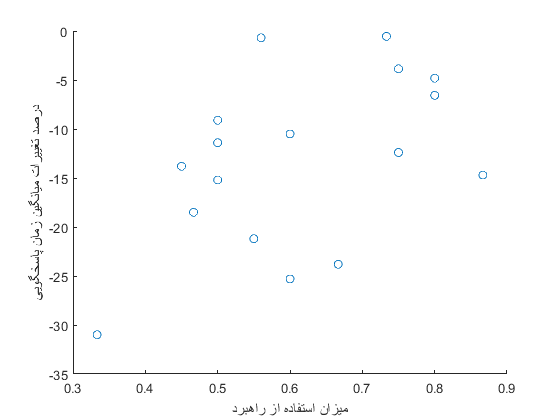
\includegraphics[scale=0.8]{Figures/stUseDtScatter.png}
\caption{\label{fig:stUseDtScatter}
نمودار نقطه‌ای مولفه $\beta$ هر بازیکن در برابر میزان استفاده‌ی وی از راهبرد
}
\end{figure}



\subsection{تحلیل آماری اختلاف میانگین‌ها}
در این قسمت قصد داریم مولفه‌های مختلف را بین گروه‌های مختلف آزمایش با هم مقایسه کنیم. به این منظور از آزمون آماری t  استفاده می‌کنیم که در آن مقدار حداقل سطح معناداری برابر با  $\alpha = 0.05$ در نظر گرفته شده است. به این منظور در هر بخش ابتدا باید بررسی کنیم شرایط آزمون t برقرار باشد. این شرایط عبارت هستند از جمع‌آوری داده‌ها به صورت تصادفی صورت گرفته باشد، هر مشاهده‌ای مستقل از سایر مشاهدات باشد و توزیع نمونه نرمال یا تقریبا نرمال باشد. دو شرط اول برای تمامی داده‌ها صدق می‌کند بنابراین شرط نرمال بودن توزیع را در هر بخش جداگانه بررسی خواهیم کرد. در صورتی که توزیع‌ها از نرمال خیلی فاصله داشته باشد از آزمون \mls{ویلکاکسون} استفاده خواهیم کرد.

\subsubsection{مقایسه عملکرد افراد در دور دوم بازی نسبت به دور اول در تمام گروه‌ها}

ابتدا توزیع عملکرد افراد در هر گروه را بررسی می‌کنیم. در شکل \ref{fig:p1sNorm} و \ref{fig:p2sNorm} و \ref{fig:p3sNorm} به ترتیب توزیع عملکرد افراد در گروه اصلی، گروه کنترل ۱ و گروه کنترل ۲ نمایش داده شده است.

\begin{figure}
\centering
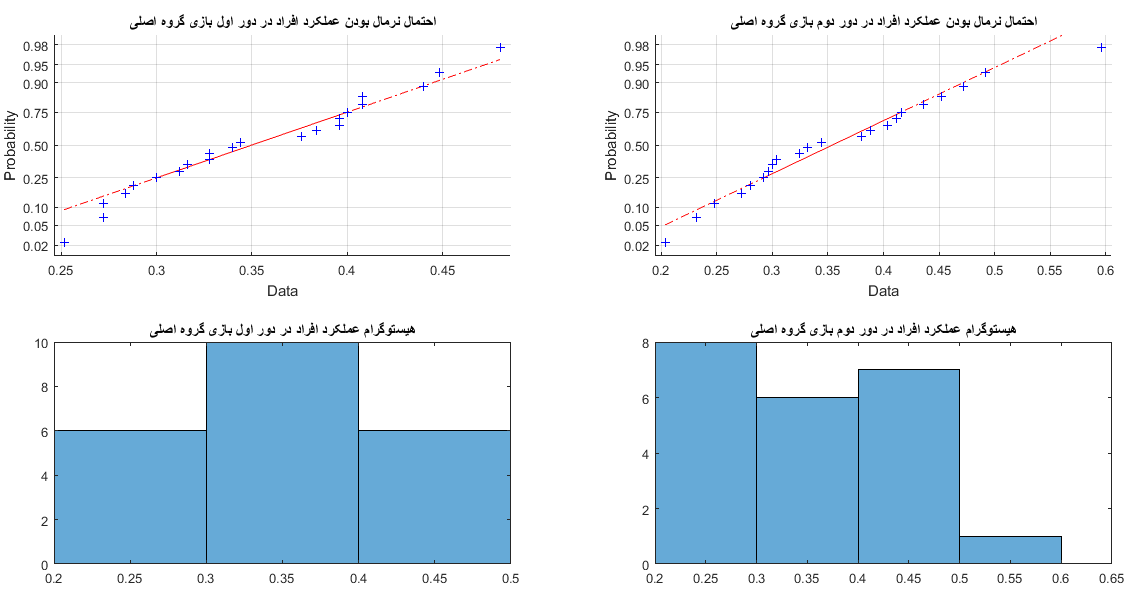
\includegraphics[scale=0.5]{Figures/p1sNorm.png}
\caption{\label{fig:p1sNorm}
نمودار احتمال نرمال بودن و هیستوگرام عملکرد گروه اصلی در دور اول و دوم بازی
}
\end{figure}

\begin{figure}
\centering
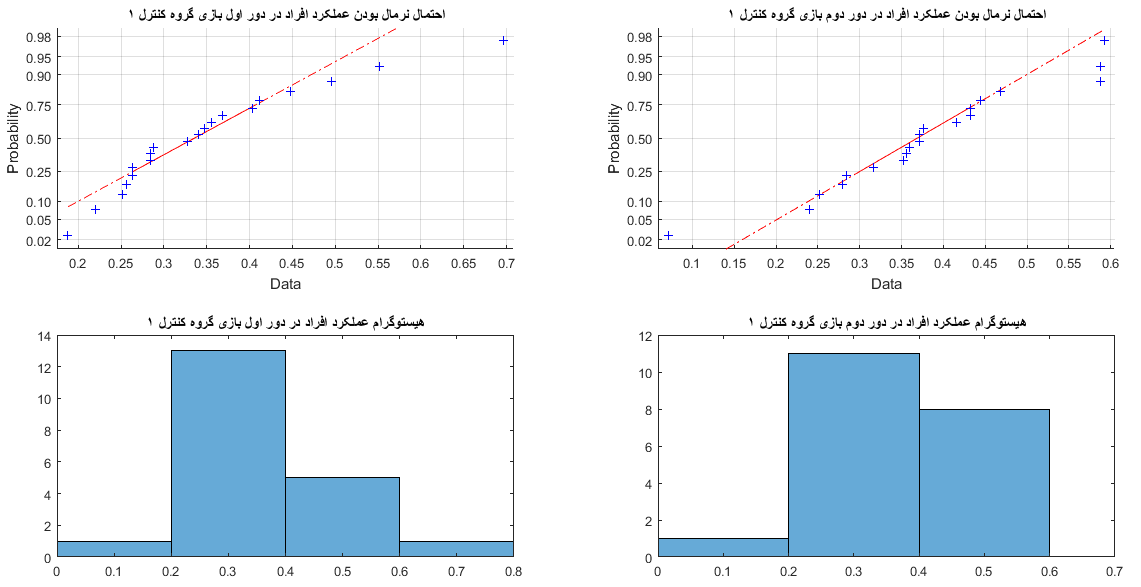
\includegraphics[scale=0.5]{Figures/p2sNorm.png}
\caption{\label{fig:p2sNorm}
نمودار احتمال نرمال بودن و هیستوگرام عملکرد گروه کنترل ۱ در دور اول و دوم بازی
}
\end{figure}

\begin{figure}
\centering
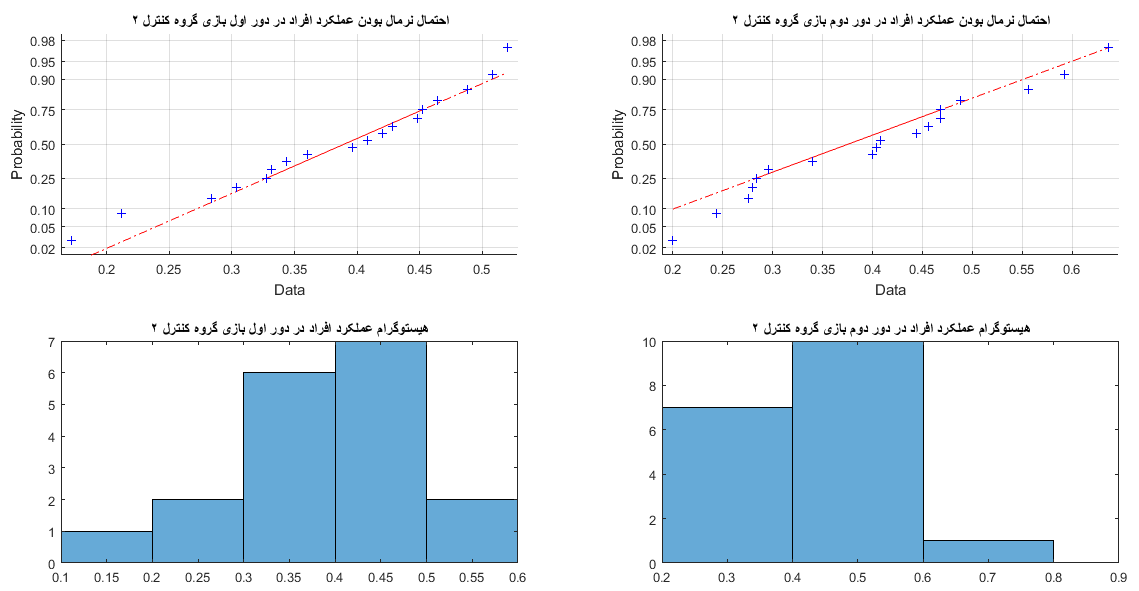
\includegraphics[scale=0.5]{Figures/p3sNorm.png}
\caption{\label{fig:p3sNorm}
نمودار احتمال نرمال بودن و هیستوگرام عملکرد گروه کنترل ۲ در دور اول و دوم بازی
}
\end{figure}

در شکل‌ها مشاهده می‌شود که توزیع‌ها به شکلی نیست که بتوانیم از روش t استفاده کنیم به همین دلیل در این قسمت از روش ویلکاکسون استفاده خواهیم کرد. نتایج به دست آمده از این روش در جدول \ref{tbl:scoreCompWilcox} نمایش داده شده است. با توجه به نتایج نمایش داده شده در جدول واضح است که در هیچ کدام از گروه‌ها عملکرد در دور دوم بازی تغییر معناداری نسبت به عملکرد در دور اول بازی نداشته است.


\begin{table}[]
\begin{scriptsize}
\begin{center}
\centering
\caption{مقایسه آماری عملکرد افراد در دور دوم بازی نسبت به دور اول}
\label{tbl:scoreCompWilcox}
\renewcommand{\arraystretch}{2}
\begin{tabular}{|c|c|c|c|}
\hline
\textbf{آزمایش}& \textbf{میانه عملکرد دور اول (درصد)} & \textbf{میانه عملکرد دور دوم (درصد)} & p-value\\ \hline
\textbf{\begin{tabular}[c]{@{}c@{}}گروه اصلی\end{tabular}} & ۳۴٪& ۳۳٪& ۰/۹۹ \\ \hline
\textbf{\begin{tabular}[c]{@{}c@{}}گروه کنترل ۱\end{tabular}} & ۳۳٪ & ۳۷٪& ۰/۲۳\\ \hline
\textbf{\begin{tabular}[c]{@{}c@{}}گروه کنترل ۲\end{tabular}} &۴۰/۲٪ & ۴۰/۶ & ۰/۷۷\\ \hline
\end{tabular}
\end{center}
\end{scriptsize}
\end{table}

موضوعی که اینجا مطرح می‌شود این است که افرادی که در دور اول بازی کردن امتیاز بالایی را کسب کرده‌اند امکان زیادی برای پیشرفت در دور دوم ندارند اما افرادی که در دور اول عملکردشان ضعیف بوده است می‌توانند پیشرفت بیشتری در دور دوم داشته باشند. به همین دلیل علاوه بر بررسی داده‌های اصلی داده‌های افرادی را که در دور اول عملکرد ضعیف‌تری داشتند را مجددا بررسی کردیم. برای این کار از هر گروه ۱۲ نفری را که عملکرد ضعیف‌تری در دور اول بازی داشتند انتخاب کردیم. نتایج به دست آمده در جدول \ref{tbl:scoreCompWilcoxWeakOnes} نمایش داده شده‌اند. با توجه به جدول مشاهده می‌شود در گروه کنترل ۱ بهبود معناداری در قسمت ۲ نسبت به قسمت ۱ مشاهده شده است ولی در گروه اصلی و گروه کنترل ۱ بهبود معناداری مشاهده نمی‌شود.

\begin{table}[]
\begin{scriptsize}
\begin{center}
\centering
\caption{مقایسه آماری عملکرد افراد ضعیف در دور دوم بازی نسبت به دور اول}
\label{tbl:scoreCompWilcoxWeakOnes}
\renewcommand{\arraystretch}{2}
\begin{tabular}{|c|c|c|c|}
\hline
\textbf{آزمایش}& \textbf{میانه عملکرد دور اول (درصد)} & \textbf{میانه عملکرد دور دوم (درصد)} & p-value\\ \hline
\textbf{\begin{tabular}[c]{@{}c@{}}گروه اصلی\end{tabular}} & ۳۰/۶٪& ۲۹/۸٪& ۰/۹۳ \\ \hline
\textbf{\begin{tabular}[c]{@{}c@{}}گروه کنترل ۱\end{tabular}} & ۲۷/۴٪ & ۳۷/۲٪& ۰/۰۱۹\\ \hline
\textbf{\begin{tabular}[c]{@{}c@{}}گروه کنترل ۲\end{tabular}} &۳۳/۸٪ & ۴۰/۶ & ۰/۳۵\\ \hline
\end{tabular}
\end{center}
\end{scriptsize}
\end{table}

\subsubsection{مقایسه‌ی تغییرات عملکرد گروه اصلی، گروه کنترل ۱ و گروه کنترل ۲}

در این بخش می‌خواهیم تغییرات عملکرد گروه اصلی، گروه کنترل ۱ و گروه کنترل ۲ را با هم مقایسه کنیم. در شکل \ref{fig:impv123NormalPlot} \mls{نمودار احتمال نرمال بودن} و \mls{هیستوگرام} برای این سه دسته از داده‌ها رسم شده است. با توجه به شکل مشاهده می‌شود که توزیع داده‌ها برای انجام دادن آزمون t مناسب است.

\begin{figure}
\centering
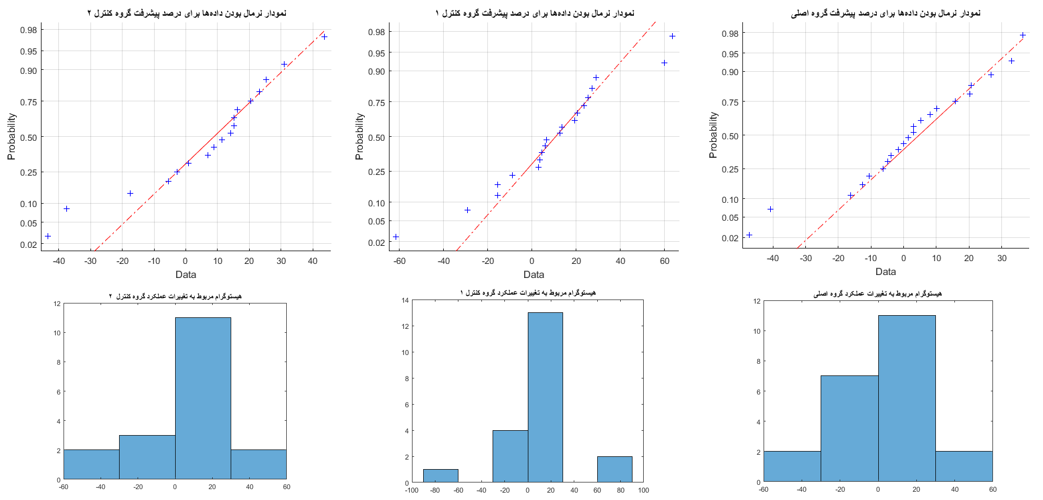
\includegraphics[scale=0.5]{Figures/impv123NormalPlot.png}
\caption{\label{fig:impv123NormalPlot}
نمودار احتمال نرمال بودن و هیستوگرام تغییرات عملکرد گروه اصلی و گروه کنترل ۱ و گروه کنترل ۲
}
\end{figure}

نتیجه‌ی به دست آمده از آزمون t در جدول \ref{tbl:impv123ttest} نمایش داده شده است. همانطور که در جدول مشاهده می‌شود مقدار p-value در تمامی موارد بیشتر از سطح معناداری است و بنابراین نمی‌توانیم نتیجه بگیریم میانگین این گروه‌ها تفاوت معناداری با یکدیگر دارند.

\begin{table}[]
\begin{scriptsize}
\begin{center}
\centering
\caption{نتایج آزمون آماری t ، مقایسه‌ی میانگین تغییرات عملکرد گروه اصلی، گروه کنترل ۱ و گروه کنترل ۲}
\label{tbl:impv123ttest}
\renewcommand{\arraystretch}{2}
\begin{tabular}{|c|c|}
\hline
\textbf{میانگین تغییرات عملکرد گروه اصلی}& ۱/۷۹٪\\ \hline
\textbf{\begin{tabular}[c]{@{}c@{}}میانگین تغییرات عملکرد گروه کنترل ۱\end{tabular}} & ۹/۳۷٪ \\ \hline
\textbf{\begin{tabular}[c]{@{}c@{}}میانگین تغییرات عملکرد گروه کنترل ۲\end{tabular}} & ۶/۹۷٪ \\ \hline
\textbf{\begin{tabular}[c]{@{}c@{}}مقدار p-value در مقایسه گروه اصلی و گروه کنترل ۱\end{tabular}} & ۰/۱۶ \\ \hline
\textbf{\begin{tabular}[c]{@{}c@{}}مقدار p-value در مقایسه گروه اصلی و گروه کنترل ۲\end{tabular}} & ۰/۲۲ \\ \hline
\textbf{\begin{tabular}[c]{@{}c@{}}مقدار p-value در مقایسه گروه کنترل ۱ و گروه کنترل ۲\end{tabular}} & ۰/۳۸ \\ \hline
\end{tabular}
\end{center}
\end{scriptsize}
\end{table}

مشابه بخش قبل با توجه به اینکه افرادی که در ابتدا عملکرد ضعیف‌تری داشته‌اند احتمال بهبود بیشتری دارند مجددا افراد ضعیف را جدا کرده و میانگین تغییرات عملکرد آنها را بررسی می‌کنیم. نتیجه‌ی این بررسی در جدول \ref{tbl:impv123ttestWeakOnes} نمایش داده شده است.

\begin{table}[]
\begin{scriptsize}
\begin{center}
\centering
\caption{نتایج آزمون آماری t ، مقایسه‌ی میانگین تغییرات عملکرد افراد ضعیف‌تر در گروه اصلی، گروه کنترل ۱ و گروه کنترل ۲}
\label{tbl:impv123ttestWeakOnes}
\renewcommand{\arraystretch}{2}
\begin{tabular}{|c|c|}
\hline
\textbf{میانگین تغییرات عملکرد گروه اصلی}& ۱/۴۴٪\\ \hline
\textbf{\begin{tabular}[c]{@{}c@{}}میانگین تغییرات عملکرد گروه کنترل ۱\end{tabular}} & ۱۸/۲۹٪ \\ \hline
\textbf{\begin{tabular}[c]{@{}c@{}}میانگین تغییرات عملکرد گروه کنترل ۲\end{tabular}} & ۷/۲۸٪ \\ \hline
\textbf{\begin{tabular}[c]{@{}c@{}}مقدار p-value در مقایسه‌ی گروه اصلی و گروه کنترل ۱\end{tabular}} & ۰/۰۳ \\ \hline
\textbf{\begin{tabular}[c]{@{}c@{}}مقدار p-value در مقایسه‌ی گروه اصلی و گروه کنترل ۲\end{tabular}} & ۰/۲۶ \\ \hline
\textbf{\begin{tabular}[c]{@{}c@{}}مقدار p-valueدر مقایسه‌ی گروه کنترل ۱ و گروه کنترل ۲\end{tabular}} & ۰/۱۴ \\ \hline
\end{tabular}
\end{center}
\end{scriptsize}
\end{table}

همانطور که مشخص است مقدار p-value در مقایسه‌ی گروه اصلی و گروه کنترل ۱ کمتر از سطح معناداری است و این به این معنا است که میانگین تغییرات عملکرد افراد ضعیف در گروه کنترل ۱ به طرز معناداری بیشتر از میانگین تغییرات عملکرد افراد ضعیف در گروه اصلی است ولی در سایر موارد تفاوت معناداری مشاهده نمی‌شود.


\subsubsection{مقایسه زمان پاسخگویی دور دوم نسبت به دور اول بازی در تمام گروه‌ها}

ابتدا باید بررسی کنیم که توزیع داده‌های مربوط به زمان به شکلی هست که بتوانیم از آزمون t استفاده کنیم یا خیر. به این منظور نمودار احتمال نرمال بودن و هیستوگرام هر بخش از داده‌ها را بررسی می‌کنیم. در شکل‌های \ref{fig:p1tNorm} و \ref{fig:p2tNorm} و \ref{fig:p3tNorm} نمودار احتمال نرمال بودن و هیستوگرام گروه اصلی، گروه کنترل ۱ و گروه کنترل ۲ به ترتیب نمایش داده شده است.

\begin{figure}
\centering
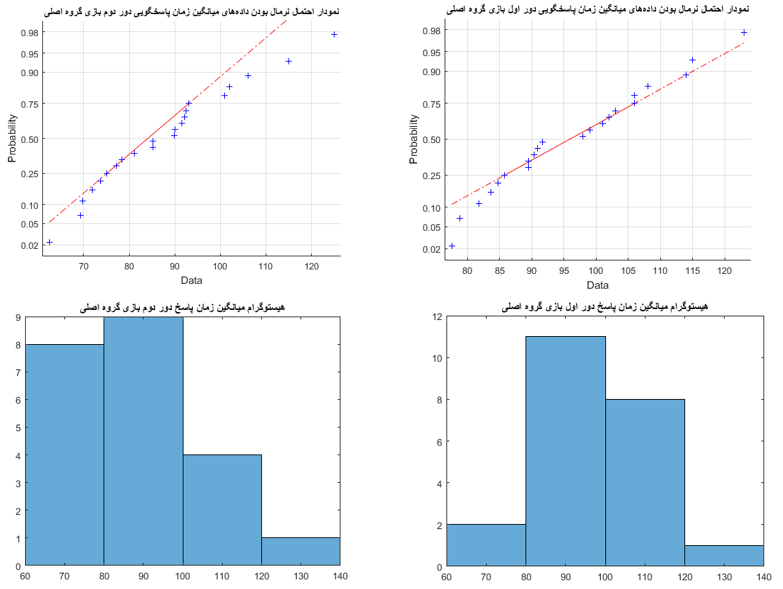
\includegraphics[scale=0.5]{Figures/p1tNorm.png}
\caption{\label{fig:p1tNorm}
نمودار احتمال نرمال بودن و هیستوگرام میانگین زمان پاسخگویی گروه اصلی
}
\end{figure}

\begin{figure}
\centering
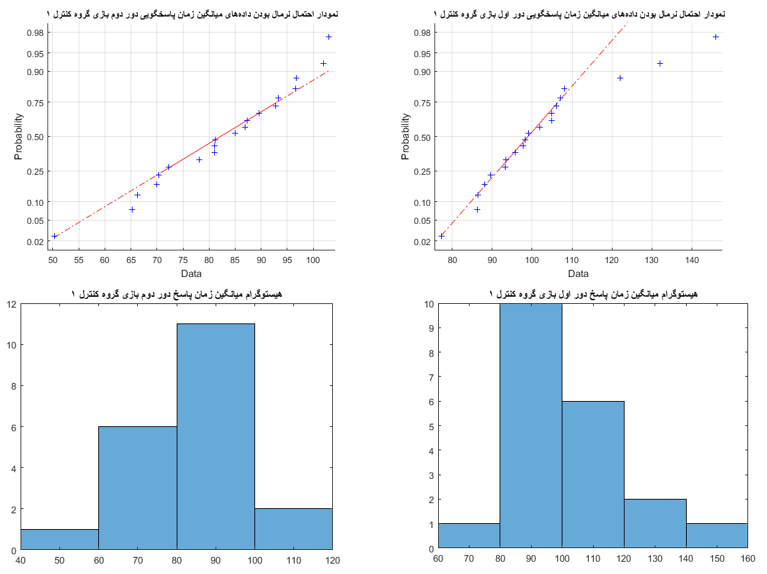
\includegraphics[scale=0.5]{Figures/p2tNorm.png}
\caption{\label{fig:p2tNorm}
نمودار احتمال نرمال بودن و هیستوگرام میانگین زمان پاسخگویی گروه کنترل ۱
}
\end{figure}

\begin{figure}
\centering
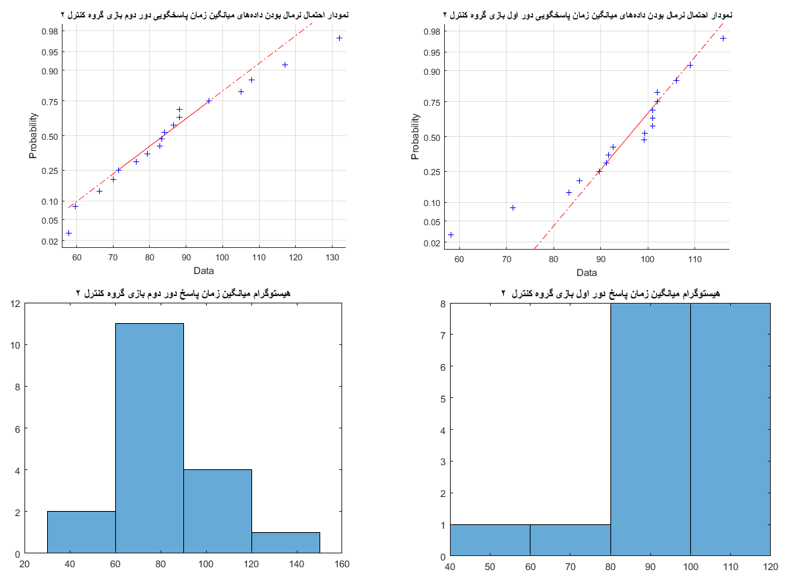
\includegraphics[scale=0.5]{Figures/p3tNorm.png}
\caption{\label{fig:p3tNorm}
نمودار احتمال نرمال بودن و هیستوگرام میانگین زمان پاسخگویی گروه کنترل ۲
}
\end{figure}

با توجه به نتایج به دست آمده در برخی از گروه‌ها توزیع داده‌ها به شکلی نیست که بتوانیم از آزمون t استفاده کنیم. بنابراین در این بخش از روش ویلکاکسون استفاده خواهیم کرد.
ابتدا زمان پاسخگویی تمام گروه‌ها در دور دوم بازی را با دور اول مقایسه می‌کنیم. نتایج این مقایسه در جدول \ref{tbl:ResponseTimeComp} نمایش داده شده است. همانطور که مشخص است با توجه به مقدار p-value میانه زمان پاسخگویی در گروه کنترل ۱ در دور دوم بازی به شکل معناداری نسبت به دور اول بازی کاهش پیدا کرده است ولی در گروه اصلی و گروه کنترل ۲ تفاوت معناداری مشاهده نمی‌کنیم.
\begin{table}[]
\begin{scriptsize}
\begin{center}
\centering
\caption{مقایسه آماری زمان پاسخگویی دور دوم بازی نسبت به دور اول}
\label{tbl:ResponseTimeComp}
\renewcommand{\arraystretch}{2}
\begin{tabular}{|c|c|c|c|}
\hline
\textbf{آزمایش}& \textbf{میانه زمان پاسخگویی دور اول (میلی ثانیه)} & \textbf{میانه زمان پاسخگویی دور دوم (میلی ثانیه)} & p-value\\ \hline
\textbf{\begin{tabular}[c]{@{}c@{}}گروه اصلی\end{tabular}} & ۹۴/۸& ۸۷/۵۵& ۰/۰۵۴ \\ \hline
\textbf{\begin{tabular}[c]{@{}c@{}}گروه کنترل ۱\end{tabular}} & ۹۸/۷ & ۸۳/۱& ۰/۰۰۰۲\\ \hline
\textbf{\begin{tabular}[c]{@{}c@{}}گروه کنترل ۲\end{tabular}} &۹۹/۲۵ & ۸۳/۶۵ & ۰/۰۶\\ \hline
\end{tabular}
\end{center}
\end{scriptsize}
\end{table}

\subsubsection{مقایسه تغییرات زمان پاسخگویی گروه اصلی، گروه کنترل ۱ و گروه کنترل ۲ نسبت به یکدیگر}
مانند بخش‌های قبل ابتدا بررسی می‌کنیم که توزیع داده‌ها مناسب استفاده از آزمون t هستند یا خیر. نمودار احتمال نرمال بودن و هیستوگرام مربوط به تغییرات زمان پاسخگویی هر سه بخش در شکل \ref{fig:dtNorm} نمایش داده شده است.

\begin{figure}
\centering
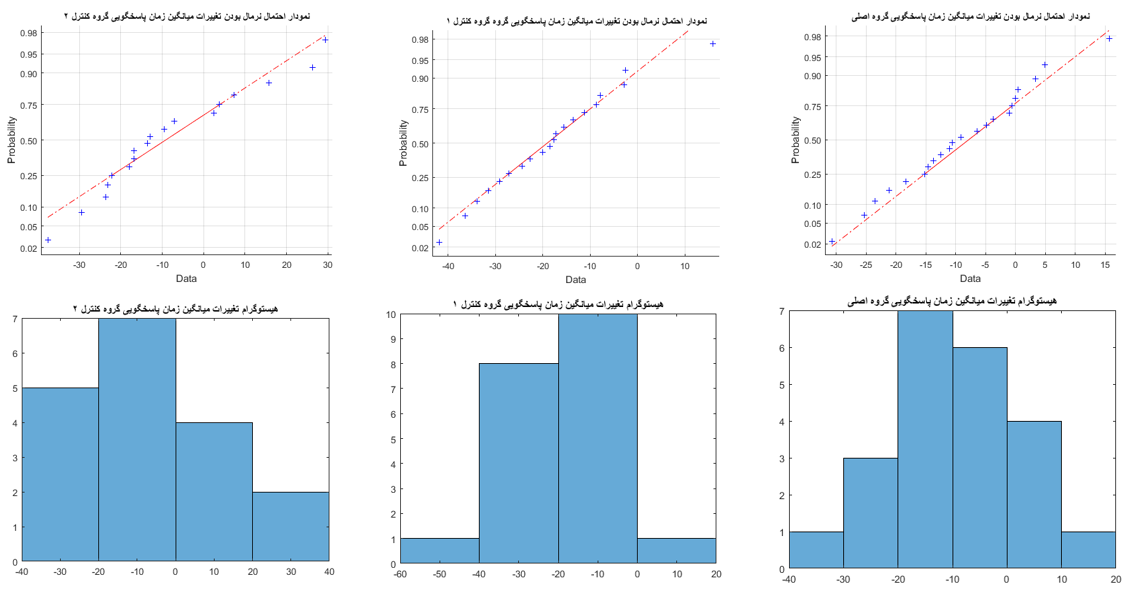
\includegraphics[scale=0.5]{Figures/dtNorm.png}
\caption{\label{fig:dtNorm}
نمودار احتمال نرمال بودن و هیستوگرام تغییرات زمان پاسخگویی هر سه گروه
}
\end{figure}

همانطور که از شکل مشخص است توزیع داده‌ها در برخی موارد به شکلی نیست که بتوانیم از آزمون t استفاده کنیم. بنابراین در این بخش از روش ویلکاکسون استفاده خواهیم کرد. نتایج در جدول \ref{tbl:dtCompWilcox} نمایش داده شده است. همانطور که از موارد نمایش داده شده در جدول مشخص است تغییرات زمان پاسخگویی گروه کنترل ۱ به طرز معناداری از تغییرات زمان پاسخگویی گروه اصلی کمتر است اما سایر موارد تفاوت معناداری با یکدیگر ندارند.

\begin{table}[]
\begin{scriptsize}
\begin{center}
\centering
\caption{نتایج آزمون ویلکاکسون، مقایسه تغییرات زمان پاسخگویی در سه گروه }
\label{tbl:dtCompWilcox}
\renewcommand{\arraystretch}{2}
\begin{tabular}{|c|c|}
\hline
\textbf{\begin{tabular}[c]{@{}c@{}}میانه تغییرات زمان پاسخگویی گروه اصلی\end{tabular}} & ۹/۸۲٪- \\ \hline
\textbf{\begin{tabular}[c]{@{}c@{}}میانه تغییرات زمان پاسخگویی گروه کنترل ۱\end{tabular}} & ۱۸/۰۱٪- \\ \hline
\textbf{\begin{tabular}[c]{@{}c@{}}میانگین تغییرات زمان پاسخگویی گروه کنترل ۲\end{tabular}} & ۱۳/۲۳٪- \\ \hline
\textbf{\begin{tabular}[c]{@{}c@{}}مقدار p-value در مقایسه‌ی گروه اصلی و گروه کنترل ۱\end{tabular}} & ۰/۰۱ \\ \hline
\textbf{\begin{tabular}[c]{@{}c@{}}مقدار p-value در مقایسه‌ی گروه اصلی و گروه کنترل ۲\end{tabular}} & ۰/۸۱ \\ \hline
\textbf{\begin{tabular}[c]{@{}c@{}}مقدار p-valueدر مقایسه‌ی گروه کنترل ۱ و گروه کنترل ۲\end{tabular}} & ۰/۰۹ \\ \hline
\end{tabular}
\end{center}
\end{scriptsize}
\end{table}

\chapter{تحلیل و جمع‌بندی}
\label{chapter:conclusion}
\thispagestyle{plain}

در این فصل به بررسی نتایج به دست آمده از آزمایش دوم می‌پردازیم.

\section{تحلیل نتایج به دست آمده}

همانطور که مشاهده کردیم آموزش راهبرد در مدت زمان محدود موجب بهبود عملکرد بازیکن‌ها نشد. در هیچ کدام از بخش‌ها بهبود معناداری بین حالتی که راهبرد آموزش داده شده و حالتی که راهبرد آموزش داده نشده است مشاهده نکردیم. گروهی که بهترین نتیجه را در مقایسه با سایر گروه‌ها داشت گروه کنترل ۱ بود. در این گروه از افراد خواسته شده راهبرد خود را گزارش کنند ولی راهبردی به آنها آموزش داده نشده است. همانطور که در فصل ۴ بررسی کردیم نتایج عملکرد افراد ضعیف این گروه بهبود معناداری در دور دوم بازی داشته است. همچنین تغییرات عملکرد افراد ضعیف این گروه به صورت معناداری از گروه اصلی (که راهبرد را آموختند) بیشتر بوده است. همچنین در مورد تغییرات زمان پاسخ، میانگین زمان پاسخ گروه کنترل ۱ در دور دوم بازی به صورت معناداری از دور اول بازی کمتر است. در نهایت تغییرات زمان پاسخ گروه کنترل ۱ به طرز معناداری از گروه اصلی کمتر است که این نشان می‌دهد افرادی که در گروه کنترل ۱ بوده‌اند توانسته‌اند بیشتر از افرادی که در گروه اصلی بوده‌اند سرعت خود را افزایش دهند. این نتایج نشان می‌دهد آگاهی نسبت به راهبردهای مورد استفاده می‌تواند باعث بهبود عملکرد افراد باشد. هرچند گروه کنترل ۱ نسبت به گروه کنترل ۲ بهبود معناداری نداشتند ولی میانگین عملکردشان بهتر از گروه ۲ بوده و میانگین زمان پاسخ‌شان کمتر از آن بوده است. همین نتایج نشان می‌دهد که این موضوع ارزش بررسی‌های بیشتر دارد.

در مورد نتایج به دست آمده از گروه اصلی می‌توان چند تحلیل ارائه داد. همانطور که مشاهده کردیم در گروه اصلی شاهد بهبود قابل توجهی نبودیم. یکی از دلایلی که می‌توان به آن اشاره کرد کم بودن زمان یادگیری است. افراد مدت زمان محدودی فرصت داشتند به یادگیری راهبرد جدید بپردازند و از آن به صورت موثر استفاده کنند. همین موضوع عامل ضعف عملکردشان است. هم باعث می‌شود نتوانند به سرعت امتیاز بیشتری کسب کنند چون در حال یادگیری یک روش جدید هستند و هم باعث می‌شود سرعت پاسخگویی‌شان یا تغییر چندانی نکند یا افزایش پیدا کند. 

\section{مشکلات موجود}

در این بخش هم مشابه بخش اول آزمایش مهم‌ترین مشکل موجود محدود بودن زمان آزمایش بود. همین موضوع باعث می‌شود راهبرد آموزش داده شده فرصت کافی برای عمیق شدن نداشته باشد. ضمن اینکه در این آزمایش تفکیکی بین افراد صورت نگرفت. به این صورت که ابتدا تعداد زیادی از افراد در یک آزمایش اولیه شرکت کنند تا سطح آنها تخمین زده شود و سپس آزمایش روی افرادی ادامه پیدا کند که سطح اولیه یکسان و ضعیف‌تری داشته‌اند. این موضوع به این دلیل حائز اهمیت است که اولا افرادی که عملکرد اولیه‌ی بهتری داشته‌اند امکان کمتری برای بهبود عملکرد دارند و ثانیا عملکرد اولیه‌ی متفاوت ممکن است روی میزان تغییر عملکرد افراد تاثیرگذار باشد و باعث شود تغییرات عملکردشان با یکدیگر قابل مقایسه نباشد.

همانند بخش قبل تعداد شرکت‌کنندگان در آزمایش کم بودند. معنادار نبودن برخی از مقایسه‌ها (مانند مقایسه گروه کنترل ۱ و گروه کنترل ۲) ممکن است به علت کم بودن افراد شرکت‌کننده در این دو آزمایش باشد.

در این پژوهش از تست پیشین و پسین استفاده نشده است. بنابراین تخمینی از وضعیت اولیه‌ی توجه افراد وجود ندارد. ممکن است همبستگی معناداری بین وضعیت اولیه‌ی توجه افراد وجود داشته باشد که در این پژوهش مغفول مانده باشد.

\section{پیشنهاداتی برای آینده}

با توجه به مشکلات موجود در این پژوهش اولین و مهم‌ترین پیشنهاد برای آینده تکرار این پژوهش با جامعه‌ی آماری بزرگتر است. در ادامه پیشنهاد می‌شود استخراج و آموزش راهبرد در طولانی مدت انجام شود. به این معنا که افراد فرصت داشته باشند طی مدت طولانی (به عنوان مثال ۱ ماه) بازی کنند و سپس راهبردهای خود را گزارش کنند. همچنین راهبرد به افراد آموزش داده شود و در جلسات تمرینی مرتب شرکت کنند و در نهایت عملکردشان با گروهی که آموزش ندیده‌اند مقایسه شود. علاوه بر این با انجام آزمایش‌هایی با تعداد شرکت‌کنندگان بیشتر از گروه کنترل ۱ و گروه کنترل ۲ این فرضیه بررسی شود که آیا گزارش راهبرد به تنهایی باعث بهبود عملکرد افراد خواهد شد یا خیر.

در پژوهش‌هایی که در سال‌های اخیر انجام شده است روی این موضوع تاکید شده است که این بازی‌ها تاثیرگذاری کوتاه‌مدت دارند ولی در طولانی مدت اثربخش نیستند (\cite{melby2013WM}). بنابراین پیشنهاد می‌شود تاثیرگذاری آموزش راهبرد پس از گذشت مدت زمان طولانی (به عنوان مثال ۲ ماه) بررسی شود.

علاوه بر این دو موضوع می‌توان به اضافه کردن یک برنامه‌ی تمرینی به بازی اشاره کرد. برنامه‌ی تمرینی به این صورت باشد که افراد قابلیت تنظیم کردن مولفه‌های مختلف بازی را داشته باشند. به عنوان مثال بتوانند تراکم ابرها، پراکندگی آنها در صفحه، تعداد ابرهای باران‌زا و عادی را تنظیم کنند و سپس مرحله‌ی تولید شده را بازی کنند.


\section{جمع‌بندی}
در این پژوهش تلاش کردیم با آموزش راهبردهای موثر یک بازی شناختی توجه به افرادی که عملکردشان ضعیف بود اثرگذاری بازی را بهبود بخشیم. دو مرحله آزمایش طراحی و پیاده‌سازی کردیم. در آزمایش اول از افراد خواستیم راهبردهای خود در بازی «ابرهای باران‌زا» را یادداشت کنند. سپس راهبردهای به دست آمده را بررسی کرده و راهبردهای موثرتر را شناسایی کردیم. در آزمایش دوم ۳ گروه را مورد بررسی قرار دادیم. هر گروه دو دور بازی کردند. از گروه اول یا همان گروه اصلی خواستیم راهبردهای خود را در دور اول گزارش کنند و در دور دوم راهبرد موثر را به آنها آموزش دادیم. از گروه دوم یا همان گروه کنترل ۱ خواستیم راهبردهای خود را در دور اول گزارش کنند ولی آموزش راهبرد صورت نگرفت. و گروه سوم یا همان گروه کنترل ۲ فقط درگیر بازی کردن شدند بدون اینکه اطلاعی از مفهوم راهبرد داشته باشند. نتایج به دست آمده نشان می‌دهد بهبود عملکرد دور دوم بازی نسبت به دور اول آن در گروه دوم معنادار بوده است. همچنین بهبود عملکرد گروه دوم نسبت به گروه اول به شکل معناداری بیشتر بوده است.

\chapter{پیوست}

\section{پیوست الف - پرسشنامه آزمایش اول} \label{attachment1}

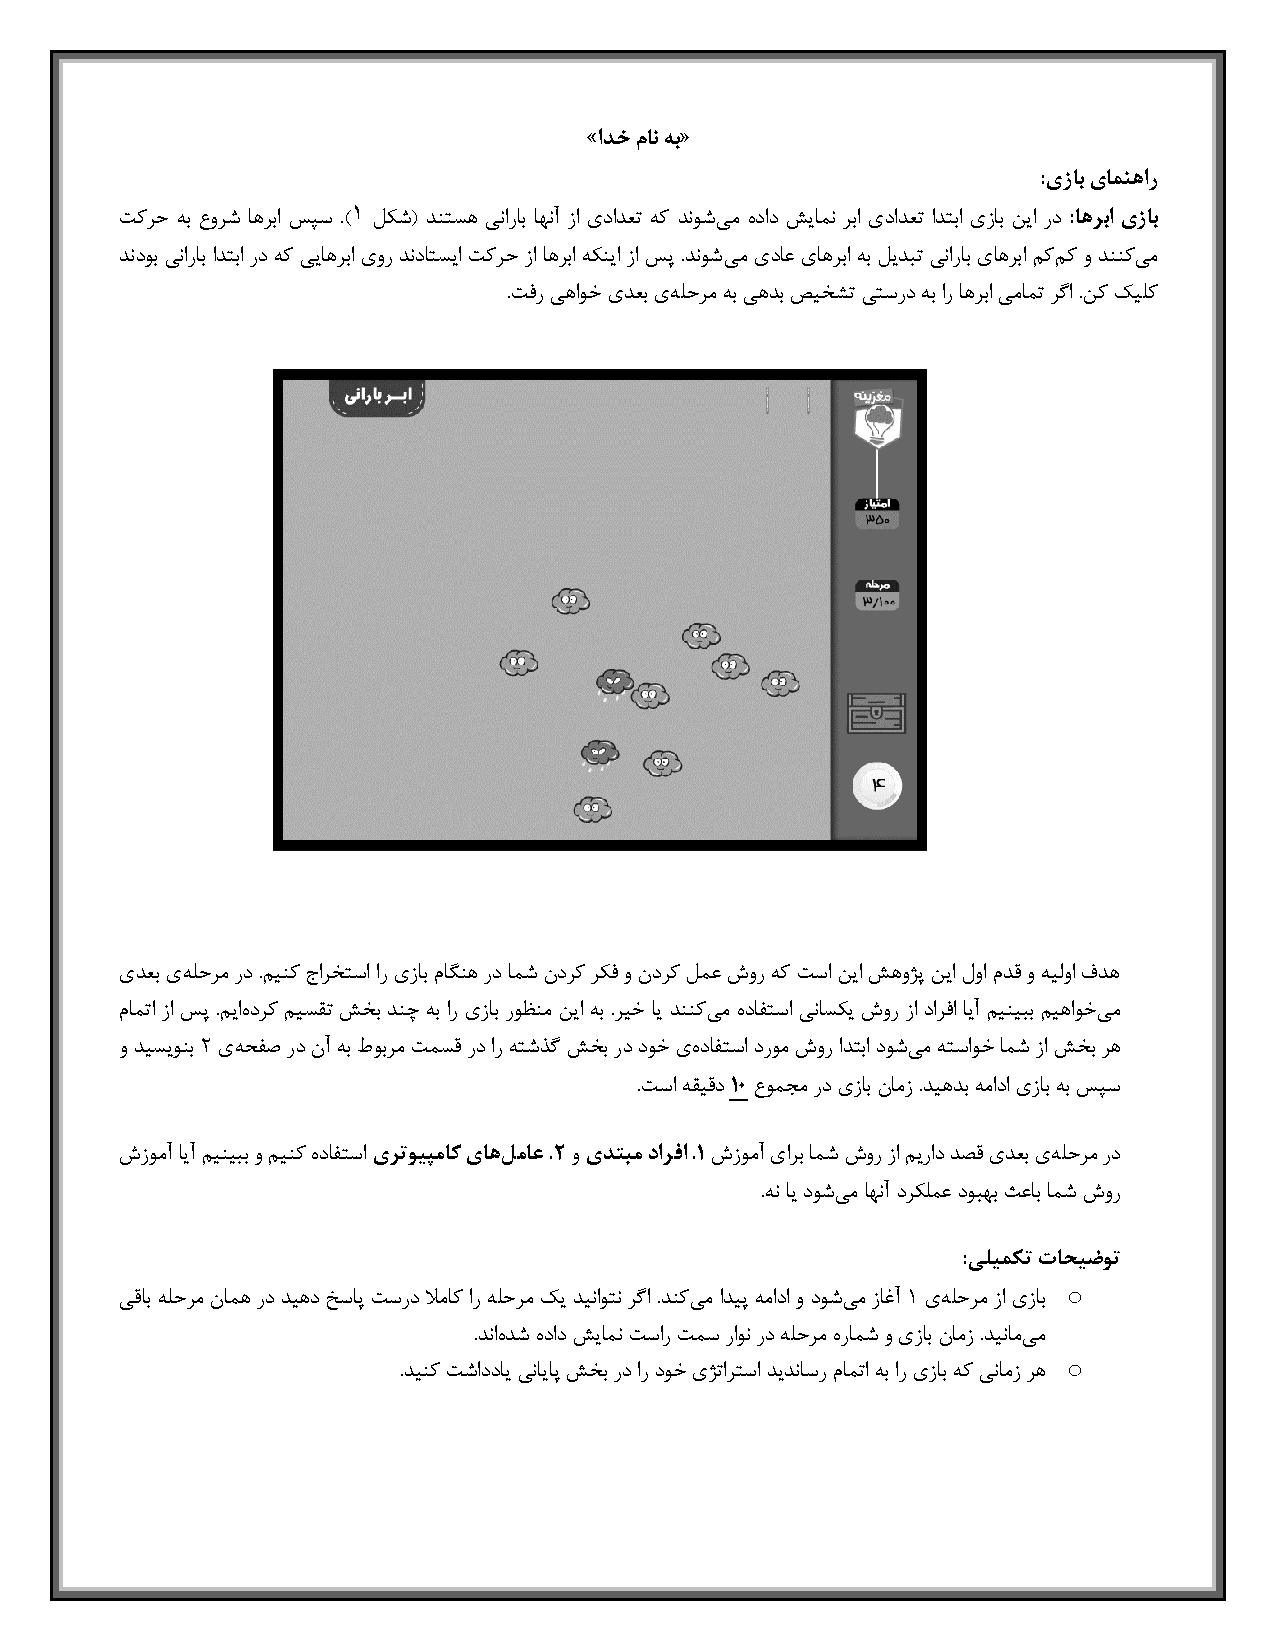
\includepdf[pages={1-4},scale=1]{docs/InformationForm_V07.pdf}

\newpage
\thispagestyle{empty}
\mbox{}

%  : \linespread{1.2}
\linespread{1}


\small{
\bibliographystyle{ieeetr-fa}
\renewcommand{\bibname}{مراجع}
\clearpage
\bibliography{ref}
\addcontentsline{toc}{chapter}{مراجع}
}

\newpage
\thispagestyle{empty}
\mbox{}
\begin{multicols}{2}
\begin{doublespace}

\glossarystyle{mylistLa}
\printglossary[type=latin]
\addcontentsline{toc}{chapter}{واژه‌نامه انگلیسی به فارسی}

\newpage
\thispagestyle{empty}
\mbox{}

\clearpage
\glossarystyle{mylistFa}
\printglossary[type=persian]
\addcontentsline{toc}{chapter}{واژه‌نامه فارسی به انگلیسی}
\end{doublespace}
\end{multicols}

\begin{latin}
\pagestyle{empty}


% LATIN ABSTRACT
\newpage
\thispagestyle{empty}
\mbox{}
\newpage
\vspace*{-2cm}
{\centering\small{\bf{Abstract}} \par \vskip .1cm}
\begin{doublespace} \normalsize

In recent years, due to the increasing amount of data available on the internet, the use of search engines to retrieve relevant information from the World Wide Web has become pervasive. Among the huge number of websites, the ones which succeed to appear more frequently and in higher ranks of search engine results would receive more visitors. So, spammers struggle to achieve a higher than deserved rank for their websites using some illegal techniques called web spamming. 
Although various methods have been used for combatting web spamming, we could basically categorize them into three groups: content-based methods, link-based methods, and the methods based on miscellaneous data. 
In this thesis, we focus on content-based and link-based methods, and also their combination.

Despite the existence of many spam detection methods, the search engines do not perform well in detecting Persian spam websites. Thus, in this thesis, after preparing a corpus of spam and non-spam Persian websites, we analyze the effectiveness of many previously proposed content-based features on detecting Persian spam websites. To improve the performance of classification, we present a number of new content-based features and examine a number of feature selection method. As another approach, we propose a new Persian spam detection system which uses an improved version of bag-of-words model and has better performance in detecting Persian web spam. Due to the prevalence of link-based spamming methods, we analyze some of these methods and propose two new algorithms which do not have the weaknesses of previous methods. In the first algorithm, to improve the process of label propagation, we use three mechanisms: optimized seed selection, edge weighting, and seed expansion. In the second algorithm, we improve the quality of websites ranking, using label propagation in both forward and backward directions. Finally, we propose a combined method, which uses the content-based probability of being spam (non-spam) to propagate the spam (non-spam) score of websites. Using this method, we increase the performance of ranking websites.
 
Finally, to evaluate the proposed methods and compare their performance with the existing methods for this task, we have conducted several experiments on different datasets. Experiment results indicate that the proposed methods have a good performance in detecting web spam.




\end{doublespace}
{\par\vspace{2mm}}
\noindent\textbf{Keywords: }\textit{Spamming, Web Spam, Spam Detection, Label Propagation, Content-Based Features}
% END OF LATIN ABSTRACT

\newpage
\mbox{}


%%%%%%%%%%%%%%%%%%%%%%%%%%%%%
% LATIN TITLE PAGE
%%%%%%%%%%%%%%%%%%%%%%%%%%%%%
\font\titlefont=cmssbx10 scaled 2074
\font\supervisorfont=cmbxti10
\newpage
\thispagestyle{empty}
\begin{center}
\begin{tabular}{lp{7cm}r}

\includegraphics[width=3.8cm]{Figures/eng.png} & & 
\includegraphics[width=2.8cm]{Figures/ut.png} \\
\end{tabular}

\vskip 1cm
\Large{\bfseries
University of Tehran \par
School of Electrical and Computer Engineering}
\large
\par
\vskip 1.5cm
\addtolength{\baselineskip}{5mm}
{\titlefont User Experience Evaluation in Attention Cognitive Game and its Usage for Improving Beginners} \par
\addtolength{\baselineskip}{-5mm}
\vskip 1cm
{\bfseries By}\par
{\Large\bfseries Elaheh Abolhassani Shahreza}\par
\vskip 1cm
Supervisors: \\
{\supervisorfont\Large Dr. Majid Nili} \\
{\supervisorfont\Large Dr. Hadi Moradi} \\
%{\supervisorfont\Large Dr. Masoud Asadpour}%
\par
\vskip 2cm
{A thesis submitted to the Graduate Studies Office \\ in partial fulfillment of the requirements \\ for the degree of Master of Science \par
in
\par
\vskip .7cm
\large Computer Engineering}
\par
\vskip .04cm
{September 2017}
\par
\vfill
\end{center}
%%%%%%%%%%%%%%%%%%%%%%%%%%%%%
% END OF LATIN TITLE

\end{latin}
\end{document}‍
